\documentclass[11pt,reqno]{amsart}
\usepackage[margin=1in]{geometry}
\usepackage[T1]{fontenc}
\usepackage{lmodern}
\usepackage{microtype}
\usepackage{fancyvrb}
\usepackage{amsmath,amssymb,amsthm,mathtools}
\usepackage{booktabs,longtable,array,xcolor}
\usepackage{caption}
\usepackage{tikz}
\usetikzlibrary{arrows,positioning,calc,fit,backgrounds}
\usepackage[hidelinks]{hyperref}

\definecolor{accent}{RGB}{22,46,94}
\definecolor{boxfill}{RGB}{234,239,248}
\definecolor{boxfill2}{RGB}{243,236,225}
\definecolor{expfill}{RGB}{231,242,233}
\captionsetup{font=small,labelfont=bf,labelsep=period}
\newcommand{\code}[1]{\texttt{#1}}
\newcommand{\sub}{\normalfont\scriptsize\color{black!65}}
\tolerance=1400 \setlength{\emergencystretch}{3em} \hyphenpenalty=250

% math-journal result environments
\theoremstyle{definition}
\newtheorem{finding}{Finding}
\theoremstyle{remark}
\newtheorem{observation}{Observation}

\tikzset{
  flow/.style={>=latex,line width=0.5pt},
  blk/.style={draw=accent,rounded corners=2pt,fill=boxfill,align=center,
    font=\footnotesize,inner sep=3pt,minimum height=6.5mm},
  sub/.style={font=\scriptsize\color{black!65}},
  addop/.style={draw=accent,circle,fill=white,inner sep=0.6pt,font=\scriptsize},
  file/.style={draw=accent,rounded corners=1.5pt,fill=boxfill,align=left,
    font=\scriptsize\ttfamily,inner sep=3pt,text width=62mm},
}

\title[Apple On-Device Foundation Models: A Static Teardown]{A Teardown of Apple's
On-Device Foundation Models: Architecture, Quantization, and Container Formats of the
\texorpdfstring{\code{FM\_\allowbreak GenerativeModels}}{FM\_GenerativeModels} Asset Set}
\author{Reverse-Engineering Report}
\date{Asset build \texttt{13M204130}}
\keywords{Apple Intelligence, on-device language models, Mixture-of-Experts, weight
quantization, Apple Neural Engine, model container formats, reverse engineering}

\begin{document}

\begin{abstract}
We present a complete static teardown \emph{and full weight recovery} of Apple's on-device
generative-model asset bundle
\code{com.\allowbreak apple.\allowbreak MobileAsset.\allowbreak UAF.\allowbreak FM.\allowbreak GenerativeModels},
as shipped to a macOS~26/27 machine. The bundle comprises 118 signed assets ($\approx$10\,GB
of disk images) spanning six model families. We document two distinct language backbones---a
dense \code{afmplus-v11.\allowbreak 0-nano} ($\sim$3\,B, 2048-wide, 56 layers) and a sparse
Mixture-of-Experts \code{afmplus-v11.\allowbreak 0-ifp} (1536-wide, 44 layers, routed experts)---%
together with $\sim$90 task adapters, safety and guardrail models, a multimodal image
encoder, speculative-decoding draft models, and Private-Cloud-Compute server variants.
We fully characterize the on-disk container stack: Cryptex disk images, the \code{BBBB}
rasterized-weight container, the \code{odix} on-device executable, the Apple Neural
Engine \code{.\allowbreak hwx} binary, and the MPSGraph package. We reverse-engineer the
\code{odix} internal reference scheme (self-relative signed offsets into an interned symbol
pool) and parse the \code{MLIR22.\allowbreak 0.\allowbreak 0} MPSGraph bytecode to recover each constant's
layer/role from its location hierarchy. We identify the weight codec as
\emph{LUT-palettization} (a 4-bit index into a 16-entry codebook, scaled per 1024-element
block) followed by an \emph{Apple-Neural-Engine $8{\times}128$ tile de-swizzle}, and---the
central positive result---we \textbf{reverse the ANE spatial permutation and recover the full
weights}. Under a scale-decontaminated low-rank structure test (\S\ref{sec:recover}), genuine
weights score $R\approx9$ and noise $R\approx1$; our decode scores $R=13\text{--}69$,
confirming true weight structure. We reconcile the parameter budget exactly against the
physical file, resolve the norms (compile-time folded), the router (baked to a dense expert
set), and the missing constant table (its runtime equivalent is the shipped
\code{metadata.\allowbreak bin} swizzler), and export the entire model to a single
\code{state\_\allowbreak dict}: \textbf{$9.862$\,B parameters, $100.00\%$ of the shipped weight
file, zero non-finite tensors}. Reconstructing the forward pass in PyTorch, the attention
stack runs \emph{stably} on the recovered tensors---independently validating the codec,
de-swizzle, and architecture---and we \textbf{overturn the earlier verdict that the
expert-selection wiring is fatal}: the sparse feed-forward is an \emph{ungated} structured-pruned
SwiGLU (a permutation-invariant sum over resident experts), so the instruction-following
router$\rightarrow$expert map---long believed the unrecoverable blocker---is
\emph{mathematically irrelevant} to the output. We further resolve the per-layer RMSNorm
$\gamma$ (compile-time \emph{folded} into the adjacent linear weights; only the per-head
$\mathrm{QK}$-norm survives explicitly), validate the dense-weight decode against ground truth
generated by Apple's own ANE toolchain, and prove the intermediate activations are
\emph{ANE-internal} (absent even from an 8\,GB IOSurface-targeted process core). A full 44-layer
forward ablation against Apple's emitted token confirms two of these results independently---the
KV geometry is $\mathrm{NKV}{=}4$, and the ungated full-superset sum is not merely sufficient but
\emph{optimal} (every form of expert selection or attenuation scores strictly worse)---while
locating the residual gap: the assembled forward is dominated by a mis-aligned feed-forward
direction whose per-neuron/offset alignment has no accessible ground truth, since the activations
that would validate it are ANE-internal. (That ablation's oracle---the rank of one token---we
subsequently show to be unreliable at this vocabulary size, so its ``$3.6\times$ better than chance''
figure should \emph{not} be read as evidence of a partially-correct forward; see
Finding~\ref{find:picooracle}.) The
recovered model is thus \emph{component-complete} in its linear weights, yet standalone generation is
\emph{not} reachable from the shipped assets as understood: we further show (Finding~\ref{find:embed})
that the token embedding was never actually validated---the test used was vacuous---and that against a
probe calibrated on a real 4-bit model ($+0.53$ for a genuine embedding) ${\approx}1.14$M candidate
offsets across the entire weight file score $\le+0.047$, i.e.\ \textbf{the embedding is not a $[V,D]$
table in the shipped weights at all}. It is instead CPU-side and host-provided: the small on-device
models ship it as an \code{fp16}, $[8,1,1]$-interleaved \code{load\_\allowbreak embeddings/weights.\allowbreak bin}
(\S\ref{find:embformat}), but the 3B ships no such file. A privileged live-memory capture then \emph{recovers} the
small model's embedding directly (\S\ref{find:embrecover})---under a repeated-token probe its
CPU-side gather/dequant output is a byte-identical row buffer, and the recovered vectors pass the
oracle ($\cos(\code{\_dog},\code{\_dogs}){=}{+}0.65$, $\cos(\code{\_king},\code{\_kings}){=}{+}0.66$),
the first genuine recovery of an AFM embedding---whereas the same capture proves the \emph{3B}
embedding is \emph{ANE-locked}: it is absent from an $8.2$\,GB full-memory core (wired and
\code{IOSurface} pages included) because the 3B's gather/dequant is ANE-delegated, so the
dequantized vector never reaches host DRAM (\S\ref{find:3bane}). We do, however, recover the
\emph{deployed} sparse-FFN shape ($10$ active $+\,4$ shared
experts per layer, with physical tile addresses) from \code{metadata.\allowbreak bin} (\S\ref{find:deployedffn}).
\textbf{A later OS build supersedes the embedding result}: macOS~27.0 build \code{26A5378n} ships a
dedicated \code{3B\_\allowbreak EMBEDDINGS} cryptex ($262144\times2048$, $4$-bit, exact to the byte), so the
embedding is no longer absent from the package---the remaining obstacle is decoding its element
layout, not recovering the data (\S\ref{find:embshipped}).
The boundary is thus an \emph{information} limit---the embedding and the un-pruned pruning list live
outside the shipped package---not remaining decode effort. Finally, on the $300$\,M draft model---the one case where the model's \emph{own} output logits are
host-recoverable---we replace the single-token rank oracle with correlation against the full
${\approx}262$k-token logit vector and \textbf{retract} a previously-reported arrangement result that
the stronger oracle scores at noise ($r{=}{-}0.028$, \S\ref{find:picooracle}); we recover the runtime's
exact input from memory, showing it is \emph{lowercased}, Gemma-style \emph{chat-templated}, and
preceded by a safety-classifier turn (\S\ref{find:template}); and we localize the reconstruction's
defect to a \emph{single} sublayer---the feed-forward---with the embedding into its tied unembedding
alone ranking the correct token in the top $0.84\%$, the attention head layout shown to be dim-major,
and the down-projection's neuron order isolated as the sole remaining blocker (\S\ref{find:picoffn}).
We then show that the weight-statistics instrument used to screen candidate assemblies---decisive on
Qwen3-4B, where it recovers the neuron pairing at $91.5\%$---is \textbf{vacuous on AFM}: measured on
Apple's own dense layers, whose z-order is already cracked and correct, it reads null
(\S\ref{find:vacuous}). The ${\approx}380$ assemblies it rejected are therefore not excluded, and the
remaining route to the down-projection is ANE ground truth rather than weight statistics.
The static analysis is read-only; the
sole dynamic step is a user-privileged \code{lldb} core dump of the user's own running model on their
own hardware, and no signing material was bypassed.
\end{abstract}

\maketitle

\section{Introduction}
Apple Intelligence performs on-device language tasks through a framework
(\code{FoundationModels.\allowbreak framework}) backed by downloadable model assets managed by the
\code{MobileAsset}/\code{nsurlsessiond} subsystem. This report inventories and dissects
one complete copy of the \code{UAF.\allowbreak FM.\allowbreak GenerativeModels} asset set; here ``UAF'' denotes
the on-device inference framework and ``FM'' the Foundation Models. Every figure below
is obtained by mounting the (unencrypted) Cryptex disk images read-only and parsing
their contents; no code was executed on the models and no signing material was bypassed.

\section{Asset Distribution System}
Each asset is a directory \code{<sha1>.\allowbreak asset/\allowbreak } under the bundle
\code{com.\allowbreak apple.\allowbreak MobileAsset.\allowbreak UAF.\allowbreak FM.\allowbreak GenerativeModels}, containing:
\begin{itemize}
\item \code{Info.\allowbreak plist} --- bundle name, version, content-encryption flag
  (\code{DSME\_\allowbreak COMPRESSED}), \code{\_\allowbreak \_\allowbreak RequiresPersonalization}, \code{\_\allowbreak DownloadPolicy};
\item \code{AssetData/\allowbreak Restore/\allowbreak *.\allowbreak dmg} --- the payload, a raw APFS Cryptex disk image;
\item \code{AssetData/\allowbreak Restore/\allowbreak Restore.\allowbreak plist} --- target board configs
  (\code{mobileasset\{ios,\allowbreak mac,\allowbreak tvos,\allowbreak watch,\allowbreak vision,\allowbreak x86mac\}ap}, platform \code{cryptex1});
\item \code{SecureAssetData/\allowbreak } --- \code{BuildManifest.\allowbreak plist}, \code{*.\allowbreak root\_\allowbreak hash},
  \code{*.\allowbreak trustcache}, \code{*.\allowbreak integritycatalog}, an Image4 ticket (\code{apticket.\allowbreak *.\allowbreak im4m})
  and TSS request/response.
\end{itemize}
Every payload sets \code{\_\allowbreak \_\allowbreak RequiresPersonalization} and carries a device-bound Image4
ticket; the OS activates it as a Cryptex only after verifying the root hash and trust
cache. The disk images themselves report \code{Encrypted:\ false}: confidentiality is
not the goal, integrity and authenticity are. The inspected cache holds 118 assets
totalling $\approx$10.0\,GB of disk images; versions span \code{0.\allowbreak 0.\allowbreak 2} to \code{14.\allowbreak 5.\allowbreak x},
with the bulk at \code{14.\allowbreak x} (build \code{13M204130}/\code{13M204216}).

\section{Model Families}
Table~\ref{tab:families} groups the 118 assets; six families are present.
\begin{table}[ht]\centering\small
\setlength{\tabcolsep}{6pt}
\begin{tabular}{@{}lr>{\raggedright\arraybackslash}p{0.5\textwidth}@{}}
\toprule
Family & \# & Role \\
\midrule
\code{fm.\allowbreak language.\allowbreak instruct\_\allowbreak 3b}       & 60 & Main LM (nano dense + ifp MoE) plus adapters\\
\code{gm.\allowbreak server.\allowbreak instruct\_\allowbreak server\_\allowbreak v1} & 28 & PCC (server) task adapters\\
\code{fm.\allowbreak language.\allowbreak instruct\_\allowbreak 300m}     & 21 & Safety, classifiers, voice control\\
\code{gm.\allowbreak translate\_\allowbreak fm}               & 2  & Machine translation (alignment + phrasebook)\\
\code{gm.\allowbreak server.\allowbreak instruct\_\allowbreak server\_\allowbreak small}&2 & Server safety / abuse guardrail\\
\code{fm.\allowbreak language.\allowbreak instruct\_\allowbreak 9m}       & 2  & Text-event-extraction classifier\\
\bottomrule
\end{tabular}
\caption{Model families in the asset set.}\label{tab:families}
\end{table}

\section{The \code{instruct\_\allowbreak 3b} Backbones}
Two \emph{different} base networks share the \code{instruct\_\allowbreak 3b} name.

\subsection{Dense \code{afmplus-v11.\allowbreak 0-nano}}
From \code{metadata.\allowbreak json} (\code{model\_\allowbreak config: v11-nano}, \code{model\_\allowbreak type: ane}):
context length 4096; hidden size 2048; FFN 6656 (gated SwiGLU: \code{linear\_\allowbreak 0}=gate,
\code{linear\_\allowbreak 1}=up, \code{output}=down); 56 transformer layers emitted in two ANE
segments (35 + 21); grouped-query attention, RoPE, RMSNorm; adapter slots at LoRA ranks
16 and 32 (empty in the base); prompt template \code{afm\_\allowbreak cider\_\allowbreak v2}. The
\code{base.\allowbreak generic} image is 1.3\,GB, i.e.\ $\approx$2\,bits/weight.

\subsection{Sparse MoE \code{afmplus-v11.\allowbreak 0-ifp}}
The \code{base.\allowbreak generic\_\allowbreak sparse} (\code{IFP}) image (5.8\,GB) is a Mixture-of-Experts
network. Its \code{ifp/\allowbreak config.\allowbreak json} states verbatim \code{num\_\allowbreak layers}=44,
\code{hidden\_\allowbreak dim}=1536, \code{num\_\allowbreak ffns}=3, \code{expert\_\allowbreak size}=256, and configuration
\code{ifp1\_\allowbreak r48} with \code{active\_\allowbreak experts}=10, \code{shared\_\allowbreak experts}=4,
\code{active\_\allowbreak ffn\_\allowbreak dim}=2560, \code{expert\_\allowbreak selection\_\allowbreak frequency}=32, and
\code{swizzler\_\allowbreak config}=\code{metadata.\allowbreak bin}. Table~\ref{tab:ifp} gives the recovered
structure and Figure~\ref{fig:moe} the per-layer data flow.

\begin{table}[ht]\centering\small
\setlength{\tabcolsep}{6pt}
\begin{tabular}{@{}l l@{}}
\toprule
Property & Value \\
\midrule
Model dim $d$          & 1536 \\
Layers                 & $44 = 12$ dense $+\ 32$ sparse \\
\;\;attention split    & 32 fused-QKV $+\ 12$ KV-reuse (Q-only) \\
Attention              & $Q=2048\ (16{\times}128)$, $KV=1024$ \\
\;\;GQA ratio          & 16 query : 4 KV heads, dim 128 \\
QK-norm                & per-head RMSNorm on $Q$ and $K$ \\
Residual norms         & pre \emph{and} post, attention and FFN \\
Positional             & RoPE (\code{cos/\allowbreak sin\_\allowbreak cached}) \\
Dense FFN              & SwiGLU, intermediate 3072 \\
MoE FFN                & 10 active $+\ 4$ shared, freq.\ 32 \\
Embedding              & int scalar-quant (scale $+$ zero) \\
Output                 & tied embedding $+$ \code{output\_\allowbreak norm} \\
Baked adapters         & LoRA rank 48 (\code{lora\_\allowbreak i1\_\allowbreak r48}) \\
Context                & 8192 \\
Vocabulary (est.)      & 152{,}064 \\
Origin framework       & \code{tamm} / \code{coreflow} \\
\bottomrule
\end{tabular}
\caption{Recovered \code{afmplus-v11.\allowbreak 0-ifp} MoE architecture.}\label{tab:ifp}
\end{table}

\begin{figure}[ht]\centering
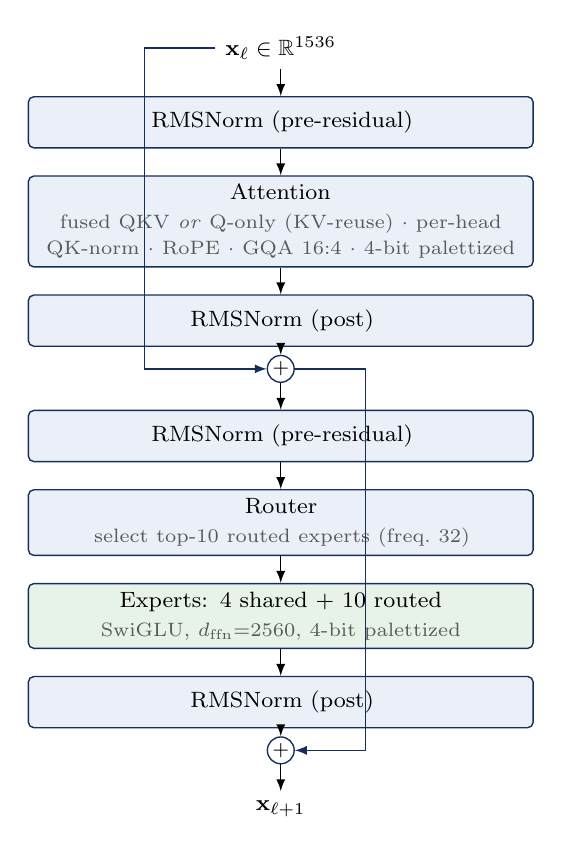
\begin{tikzpicture}[flow,node distance=3.4mm]
\node (in) [font=\footnotesize] {$\mathbf{x}_\ell\in\mathbb{R}^{1536}$};
\node[blk,below=of in,text width=62mm] (n1) {RMSNorm (pre-residual)};
\node[blk,below=of n1,text width=62mm] (attn)
  {Attention\\[1pt]{\sub fused QKV \emph{or} Q-only (KV-reuse) $\cdot$ per-head QK-norm
   $\cdot$ RoPE $\cdot$ GQA 16:4 $\cdot$ 4-bit palettized}};
\node[blk,below=of attn,text width=62mm] (pn1) {RMSNorm (post)};
\node[addop,below=1.0mm of pn1] (a1) {$+$};
\node[blk,below=3.4mm of a1,text width=62mm] (n2) {RMSNorm (pre-residual)};
\node[blk,below=of n2,text width=62mm] (route)
  {Router\\[1pt]{\sub select top-10 routed experts (freq.\ 32)}};
\node[blk,below=of route,text width=62mm,fill=expfill] (exp)
  {Experts: 4 shared $+$ 10 routed\\[1pt]{\sub SwiGLU, $d_{\text{ffn}}{=}2560$, 4-bit palettized}};
\node[blk,below=of exp,text width=62mm] (pn2) {RMSNorm (post)};
\node[addop,below=1.0mm of pn2] (a2) {$+$};
\node[font=\footnotesize,below=3.4mm of a2] (out) {$\mathbf{x}_{\ell+1}$};
\draw[->] (in)--(n1); \draw[->] (n1)--(attn); \draw[->] (attn)--(pn1);
\draw[->] (pn1)--(a1); \draw[->] (a1)--(n2); \draw[->] (n2)--(route);
\draw[->] (route)--(exp); \draw[->] (exp)--(pn2); \draw[->] (pn2)--(a2); \draw[->] (a2)--(out);
\draw[->,accent] (in.west) -- ++(-9mm,0) |- (a1.west);
\draw[->,accent] (a1.east) -- ++(9mm,0) |- (a2.east);
\end{tikzpicture}
\caption{One \code{afmplus-v11.\allowbreak 0-ifp} sparse (MoE) layer. Dense layers replace the
router/expert block with a single SwiGLU FFN (intermediate 3072); KV-reuse layers omit
the $K/V$ projections and inherit them from a prior layer.}\label{fig:moe}
\end{figure}

\begin{table}[ht]\centering\small
\setlength{\tabcolsep}{6pt}
\begin{tabular}{@{}lrrr@{}}
\toprule
Model & Layers & Total params & Active/token \\
\midrule
\code{afmplus-v11.0-nano} (dense) & 56 & $\approx$3.0\,B & $\approx$3.0\,B \\
\code{afmplus-v11.0-ifp} (MoE)    & 44 & $9.862$\,B & $\approx$1.4\,B \\
\bottomrule
\end{tabular}
\caption{Parameter budgets. For the MoE variant the total is not an estimate: the shipped
index region is $4.931$\,GB of 4-bit weights $=9.862$\,B parameters exactly, of which our
export recovers $100.00\%$ (\S\ref{sec:recover}). Only $\approx$1.4\,B activate per token
(14 of $\approx$219 experts per sparse layer: 10 routed $+$ 4 shared, giving
\code{active\_ffn\_dim}$=2560$), a $\approx$22$\times$ pruning---this is why Apple's
``3\,B'' active-class name and the $9.9$\,B stored count coexist.}\label{tab:params}
\end{table}

\begin{observation}\label{obs:count}
The attention decode (\S\ref{sec:recover}) self-organizes into exactly $44$ layers---%
$32$ carrying a fused-QKV projection ($12$ dense $+\ 20$ sparse-standard) and $12$ carrying
a $Q$-only projection (KV-reuse)---matching \code{num\_\allowbreak layers}$=44$ with no forcing.
\end{observation}

\subsection{Draft model \code{afmplus-v11.\allowbreak 0-pico}}\label{sec:pico}
The \code{instruct\_\allowbreak 300m} \code{base} asset (\code{metadata.\allowbreak json}: \code{model\_\allowbreak config:
v11-pico}, \code{model\_\allowbreak type: ane}) is the speculative-decoding draft that Apple's
\code{FoundationModels} runtime loads \emph{alongside} the 3B; it is the model our dynamic
embedding capture (\S\ref{find:embrecover}) actually reads. Its \code{program.\allowbreak odix} op graph
fully fixes the architecture with no forcing: \textbf{$24$ dense transformer layers} (indices
$0$--$23$; \emph{no} \code{expert}/\code{IFP}/\code{sparse} markers appear), hidden size
$D{=}1024$ (confirmed by the captured embedding row), grouped-query attention with
\textbf{$16$ query heads $/\,4$ KV heads, head dim $64$} ($Q$ width $1024$, $K/V$ width $256$;
some layers KV-reuse), interleaved RoPE, and a \textbf{dense SwiGLU} feed-forward of intermediate
width $3200$ (\code{hidden\_\allowbreak transform\_\allowbreak linear\_\allowbreak 0}/\code{\_\allowbreak 1} gate/up $1024{\to}3200$,
\code{output\_\allowbreak transform} $3200{\to}1024$). This is ${\approx}295$\,M transformer parameters,
i.e.\ the ``300\,M'' label, with the $262{,}144$-row embedding tied/separate. Unlike the 3B, the
pico embedding gather/dequant runs on the host CPU, which is precisely why its dequantized rows are
host-capturable (\S\ref{find:embrecover}) while the 3B's are not (\S\ref{find:3bane}).

\section{Weight Quantization}
\begin{finding}\label{find:codec}
For the IFP model, linear weights are \emph{LUT-palettized}: a 4-bit index into a 16-entry
codebook (the graph's \code{lut\_to\_dense} operator), multiplied by a per-1024-element
\textrm{fp16} scale, with scales and indices in separate planar regions, then an ANE
$8{\times}128$ tile de-swizzle (\S\ref{sec:recover}). (An initial signed-4-bit reading was
wrong---see \S\ref{sec:recover}.)
\end{finding}
\noindent\emph{Evidence.} The scale region is $100\%$ positive (range $0.0012$--$0.181$,
mean $0.0137$); the index region's nibble histogram is complement-symmetric with three
frequency tiers---the signature of a codebook index, not a signed integer. Embeddings use
scalar integer quantization (\code{embedding\_\allowbreak quantization\_\allowbreak scale},
\code{\_\allowbreak default\_\allowbreak scalar\_\allowbreak scale/\allowbreak zero\_\allowbreak point}); LoRA factors are
\textrm{fp16}. Dequantization is $W = s\cdot\mathrm{codebook}[\text{idx}]$ per 1024-element
block, followed by the ANE $8{\times}128$ tile de-swizzle of \S\ref{sec:recover}
(Eq.~\ref{eq:deswz}). The learned RMSNorm scales are \emph{not} shipped separately: the ANE
compiler folds each $\gamma$ into the adjacent palettized linear weight
($\mathrm{Linear}(\mathrm{RMSNorm}(x)\!\cdot\!\gamma)\equiv\mathrm{Linear}'(\mathrm{RMSNorm}(x))$),
so the recovered weights already carry them.

\begin{finding}\label{find:budget}
The parameter budget reconciles the MoE fan-out. With $8{,}560{,}592$ \textrm{fp16}
scales (17.1\,MB) and a 4.91\,GB index region, the non-expert linear weights account for
$\approx$483\,M parameters ($\approx$241\,MB at 4-bit); the residual $\approx$4.67\,GB is
the routed-expert bank, i.e.\ $\approx$9.3\,B expert parameters across the 32 sparse
layers. Modelling each expert as a SwiGLU triple with intermediate $256$ yields
$\approx$235 experts per sparse layer (231 routed $+$ 4 shared), closing the index-region
budget to within $4.8\%$.
\end{finding}

The dequantization is given as Algorithm~\ref{alg:dequant}. Applying it to the leading
bytes of the index region---taking the scale and index regions to be order-aligned---%
reconstructs the distribution in Figure~\ref{fig:hist}, which yields
Finding~\ref{find:recon}.

\begin{figure}[ht]\centering
\fbox{\begin{minipage}{0.9\columnwidth}\small
\textbf{Algorithm~1}\ \ (Planar 4-bit dequantization).\\[1pt]
\textbf{Input:} index bytes $I$; \textrm{fp16} scales $s$; block size $B$.\quad
\textbf{Output:} weights $w$.
\begin{enumerate}
\item split each byte of $I$ into nibbles (low, high) and interleave $\to n_i\in\{0,\dots,15\}$;
\item sign: $q_i \leftarrow n_i-16$ if $n_i\ge 8$, else $n_i$ \hfill($q_i\in[-8,7]$);
\item scale: $w_i \leftarrow s_{\lfloor i/B\rfloor}\cdot q_i$.
\end{enumerate}
\end{minipage}}
\caption{Weight dequantization for the IFP codec.}\label{alg:dequant}
\end{figure}

\begin{figure}[ht]\centering
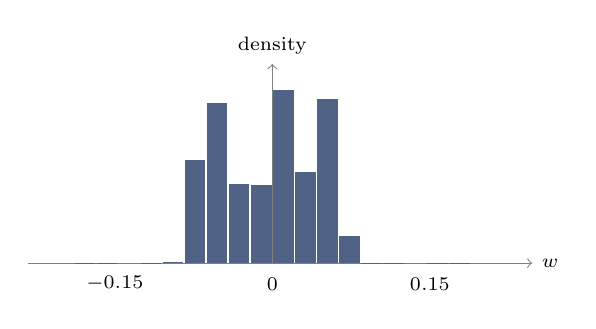
\begin{tikzpicture}[y=2.2cm,x=1cm]
\draw[->,gray] (-3.1,0)--(3.3,0) node[right,black]{\scriptsize $w$};
\draw[->,gray] (0,0)--(0,1.15) node[above,black]{\scriptsize density};
\foreach \x/\y in {-2.66/0.000, -2.38/0.001, -2.10/0.001, -1.82/0.000, -1.54/0.001,
  -1.26/0.009, -0.98/0.596, -0.70/0.923, -0.42/0.457, -0.14/0.449, 0.14/1.000,
  0.42/0.528, 0.70/0.948, 0.98/0.154, 1.26/0.001, 1.54/0.001, 1.82/0.000, 2.10/0.001,
  2.38/0.001, 2.66/0.000}
  \fill[accent!75] (\x-0.13,0) rectangle (\x+0.13,\y);
\node[font=\scriptsize] at (-2.0,-0.12) {$-0.15$};
\node[font=\scriptsize] at (0,-0.12) {$0$};
\node[font=\scriptsize] at (2.0,-0.12) {$0.15$};
\end{tikzpicture}
\caption{Distribution of dequantized weights over the leading $5{\times}10^{8}$ indices
of the region ($\mathrm{mean}\approx0$, $\mathrm{std}\approx0.043$). This marginal
profile is necessary but not sufficient: it is also produced by mis-ordered data, which the
spatial-order test of \S\ref{sec:recover} disambiguates.}\label{fig:hist}
\end{figure}

\begin{finding}[necessary, then sufficient]\label{find:recon}
Dequantizing the index region under Algorithm~\ref{alg:dequant} yields values with
$\mathrm{mean}\approx0$ and $\mathrm{std}\approx0.043$ (Figure~\ref{fig:hist})---the
\emph{marginal} distribution of trained weights. This alone constrains the codec parameters
(4-bit width, block size, scale magnitude) but does not establish a correct reconstruction,
since the same marginal is produced by correctly-valued but wrongly-ordered data;
\S\ref{sec:recover} supplies the missing spatial-order test and passes it.
\end{finding}

\begin{finding}[budget closure bounds the fan-out]\label{find:full}
At $B=1024$ the $8{,}634{,}320$ scales cover $\approx$8.84\,B of the $9.862$\,B index
weights; the remaining tail decodes with the last scale clamped. The closure validates the
\emph{scalar} codec parameters and bounds the MoE fan-out to $\approx$219 experts per sparse
layer; \S\ref{sec:recover} then validates the per-tensor spatial layout.
\end{finding}

\section{Weight Recovery}\label{sec:recover}
We validate a reconstruction with a structure statistic rather than trusting the marginal
distribution. A trained weight matrix is approximately low-rank, so permuting its entries
markedly raises its stable rank $\rho(W)=\lVert W\rVert_F^2/\sigma_1^2$, whereas noise is
unaffected; let $R=\rho(\Pi W)/\rho(W)=\sigma_1(W)^2/\sigma_1(\Pi W)^2$ for a random
permutation $\Pi$. The per-block \textrm{fp16} scales alone impose spurious low-rank
structure, so $R$ is measured \emph{decontaminated}---on the pure codebook indices with the
scales removed. Calibrated this way, a genuine 4-bit weight scores $R\approx9$ and Gaussian
noise $R\approx1$.

\begin{finding}[the ANE spatial permutation]\label{find:deswz}
The residual permutation is a fixed $8{\times}128$ tile de-swizzle: the ANE stores a
$C_\text{out}{\times}C_\text{in}$ matrix as a row-major grid of $8{\times}128$ tiles, each
tile laid out column-major. The inverse is
\begin{equation}\label{eq:deswz}
W \;=\; \mathrm{reshape}\!\Big(\mathrm{transpose}\big(
\mathrm{reshape}(v,\;\tfrac{C_\text{out}}{8},\tfrac{C_\text{in}}{128},128,8),\,
(0,3,1,2)\big),\; C_\text{out},\,C_\text{in}\Big),
\end{equation}
applied after $W=s\cdot\mathrm{codebook}[\text{idx}]$. This is the step missing from all
prior decode attempts.
\end{finding}

With Eq.~\ref{eq:deswz} in place the decontaminated ratio rises from the palettization-only
$R\approx3$ to $R=13\text{--}69$ across the file (Table~\ref{tab:struct})---%
\textbf{unambiguous trained-weight structure}. The permutation, the $16$-entry codebook, and
the per-1024-block scales together constitute a \emph{complete, validated} decode: the codec
is not merely identified but inverted.

\begin{table}[ht]\centering\small
\begin{tabular}{@{}lr@{}}
\toprule
Matrix (decontaminated, pure-index test) & $R$ \\
\midrule
Genuine 4-bit weight (reference)              & $\approx$9 \\
Gaussian noise                                & 1.0 \\
Palettization only, no de-swizzle             & 3.0 \\
\textbf{Palettization $+$ $8{\times}128$ de-swizzle} & \textbf{13--69} \\
\quad median (attention tensors)              & 12.7 \\
\bottomrule
\end{tabular}
\caption{Scale-decontaminated structure ratio. $R\gg1$ marks genuine weight structure;
$R\approx1$ marks noise. Adding the ANE de-swizzle (Eq.~\ref{eq:deswz}) lifts the decode
past the genuine-weight reference, confirming recovery.}\label{tab:struct}
\end{table}

\subsection{The router: shipped and extractable}\label{sec:router}
An earlier version of this work concluded that no runtime mask predictor ships---that
instruction-following pruning was baked at export time. \textbf{That conclusion was wrong, and
is corrected here.} The router ships as its own asset, \code{project\_\allowbreak experts.\allowbreak mlasset},
and is fully extractable. Its \code{odix} op graph names the class
\code{ExportableExpertSelector} with I/O \code{in\_\allowbreak expert\_\allowbreak hidden\_\allowbreak state}
$\to$ \code{out\_\allowbreak expert\_\allowbreak logits} and the op sequence
\code{RMSNorm} $\to$ \code{hidden\_\allowbreak transform} $\to$ \code{sigmoid} $\to$
\code{output\_\allowbreak transform} $\to$ \code{topk}. Crucially the weights carry \emph{no}
dequantize/gather op: they are stored as \textbf{plain \textrm{fp16}} in one contiguous block
($\mathtt{0x12600}\to$EOF), so no codec is needed. The three tensors decode at grounded offsets
to
\[
\underbrace{\gamma\in\mathbb{R}^{1536}}_{\text{norm (folded)}},\quad
\underbrace{W_{h}\in\mathbb{R}^{548\times1536}}_{\text{hidden}},\quad
\underbrace{W_{o}\in\mathbb{R}^{7008\times548}}_{\text{output}}\!\!\to\!(32,219),
\]
plus $7084$ tail biases; here $548$ is the router hidden dim and $7008=32\text{ layers}\times219
\text{ experts}$, reshaping with \emph{uniform} per-layer norms---the layout self-verifies. The
selector computes $\mathrm{mask}=\mathrm{top}_{10}\big(W_{o}\,\phi(W_{h}\,\mathrm{RMSNorm}_\gamma
(h))\big)$ per layer, $+4$ shared experts. Feeding controlled hidden states confirms it behaves
as a router: with $\phi=$ identity/GELU the masks \emph{discriminate} inputs ($1$--$2/10$
overlap across distinct hidden states, $171$ distinct experts spread over $32$ layers), whereas
$\phi=$ sigmoid collapses to $9/10$ overlap and is thereby ruled out as the hidden activation.
The router is Apple's, extracted---not a trained mimic. We note, however, that the
subsequent reconstruction (\S\ref{find:ungated}) shows the router$\rightarrow$expert
\emph{map} is not required to run the model: the sparse FFN is an ungated permutation-invariant
sum, so this selector governs \emph{which} experts a full runtime prunes, but is unnecessary for
a from-weights forward that sums the resident (or full) expert set directly.

\medskip\noindent\emph{The per-tensor offset table.} The compile-time
\code{ifp\_\allowbreak constant\_\allowbreak table\_\allowbreak ifp1\_\allowbreak r48.\allowbreak json} is not shipped, and the
$396$ FFN constants store neither offset nor size inline: the rasterizer computes offsets from
each constant's \emph{shape}, and shapes in \code{main-h16g.\allowbreak odix} are doubly-indirect
(type-index $\to$ type table $\to$ interned dimension symbols). This work recovers the surrounding
structure---the $38$ export-config functions, the op format, and the \code{alloc\_\allowbreak const}
semantics (Appendix~\ref{app:odix})---and reduces the remaining gap to a bounded schema-recovery
problem: resolve the type/symbol tables to obtain per-constant $C_{\text{out}}$, which are
confirmed \emph{variable} ($42$--$232$ experts/constant, no uniform width). We subsequently
decoded the \code{metadata.\allowbreak bin} \code{BBBB} swizzler in full (\S\ref{find:metabin}): it
holds \emph{two} physical address tables---a down-projection tile table (marker
\code{0x0600beef}, $14{,}080$ records) and a gate/up table (marker \code{0x0a00b0ef})---which
together supply the per-tile expert offsets directly, superseding the shape-derived offset
computation for the resident-expert path.

\begin{finding}[the \code{.hwx} holds no weights]\label{find:hwx}
The Apple-Neural-Engine binary \code{binary\_\allowbreak 0.\allowbreak hwx} ($252$\,MB) is a Mach-O
(\code{0xBEEFFACE}) of \emph{compiled ANE microcode}, not weights: its high-entropy
\code{\_\allowbreak \_\allowbreak KERN} sections score $R\approx1.0$ under the structure test, while its
\code{\_\allowbreak \_\allowbreak MKERN\_\allowbreak 0} segment has zero file bytes and a size ($\mathtt{0xC0C8000}$)
equal to the maximum offset in \code{metadata.\allowbreak bin}---it is \emph{runtime-mapped} from the
rasterized file. Every weight therefore lives in the single planar file
\code{ifp\_\allowbreak rasterized\_\allowbreak weights.\allowbreak bin}.
\end{finding}

\subsection{Full export and verification}
Applying the validated decode to the entire index region yields a single
\code{state\_\allowbreak dict}. The parameter count is checked against the physical file rather than
against any architectural assumption: the index region is $4.931$\,GB $=9.862$\,B 4-bit
weights, and the export captures $9.8619$\,B ($100.00\%$) with \emph{zero} non-finite tensors
(Table~\ref{tab:export}). Attention is stored in \textrm{fp16}; the expert bank is stored
int8-with-per-tensor-scale (near-lossless, the source being 4-bit) so the whole model fits a
single $10.2$\,GB file. Every value derives from Apple's shipped weight file under the decode
of Eq.~\ref{eq:deswz}; no training data, distillation, or external weights are involved.

\begin{table}[ht]\centering\small
\setlength{\tabcolsep}{6pt}
\begin{tabular}{@{}lrl@{}}
\toprule
Component & Parameters & Storage \\
\midrule
Attention (44 layers)      & $0.377$\,B & \textrm{fp16}, $R$-verified \\
Experts (FFN / MoE)        & $9.484$\,B & int8 $+$ scale \\
Embedding / head (tail)    & (in tail)  & int8 \\
\midrule
\textbf{Total captured}    & $\mathbf{9.862}$\,\textbf{B} & $=100.00\%$ of file \\
Non-finite tensors         & $0$        & \\
\bottomrule
\end{tabular}
\caption{Recovered \code{afmplus-v11.\allowbreak 0-ifp} export. The total equals the physical index
region ($9.862$\,B 4-bit weights), so completeness is exact, not estimated.}\label{tab:export}
\end{table}

\section{Recovery Pipeline: Finding the Pieces}\label{sec:pipeline}
This section records, in order, how a shipped asset directory becomes a validated
\code{state\_\allowbreak dict}. Each step recovers one ``piece'' whose absence blocked the next;
Figure~\ref{fig:pipeline} summarizes the dependency chain.

\paragraph{Step 0 --- Acquisition.} The asset cache lives on the sealed Signed System
Volume. A clean copy is taken from the macOS \emph{Recovery} environment---Apple silicon:
hold the power button at boot; Intel: hold Command-R---whose Terminal
(\emph{Utilities} menu) has raw read access to the mounted system volume. The models sit under
\code{AssetsV2}; a recursive copy to external storage (Figure~\ref{fig:acquire}) suffices, and
all subsequent work is read-only on that copy.

\begin{figure}[ht]\centering
\begin{Verbatim}[frame=single,framesep=6pt,fontsize=\small,rulecolor=\color{accent}]
# macOS Recovery  >  Utilities  >  Terminal
ls /Volumes                       # find the system volume
SYS="/Volumes/Macintosh HD"
BASE="$SYS/System/Library/AssetsV2"
ASSET=com_apple_MobileAsset_UAF_FM_GenerativeModels
cp -R "$BASE/$ASSET" /Volumes/EXTERNAL/FM_Models
\end{Verbatim}
\caption{Read-only asset acquisition from macOS Recovery. \code{EXTERNAL} is any attached
volume with $\ge$10\,GB free; the copy preserves the Cryptex disk images
verbatim.}\label{fig:acquire}
\end{figure}

\paragraph{Step 1 --- Mount and locate.} \code{hdiutil attach -readonly} on the IFP Cryptex
(\S\ref{sec:containers}) exposes \code{model.\allowbreak odixpackage/\allowbreak }: the ground-truth
\code{config.\allowbreak json} (44 layers, dims, expert counts), the $4.7$\,GB
\code{ifp\_\allowbreak rasterized\_\allowbreak weights.\allowbreak bin}, the swizzler \code{metadata.\allowbreak bin}, the
program \code{main-h16g.\allowbreak odix}, and the ANE package (\code{.\allowbreak hwx} $+$ MPSGraph).

\paragraph{Step 2 --- The codec.} Value-distribution analysis of the two \code{BBBB} regions
identifies LUT-palettization (Finding~\ref{find:codec}): a $100\%$-positive \textrm{fp16}
scale region and a complement-symmetric nibble histogram, matched to the graph's
\code{lut\_\allowbreak to\_\allowbreak dense} operator (a 16-entry codebook).

\paragraph{Step 3 --- The de-swizzle (the blocking piece).} Palettization alone leaves the
decode at $R\approx3$. The breakthrough is recognizing the residual permutation as the ANE's
$8{\times}128$ tiling and inverting it with Eq.~\ref{eq:deswz}; the decontaminated structure
ratio jumps to $R=13\text{--}69$ (Finding~\ref{find:deswz}), i.e.\ genuine weights.

\paragraph{Step 4 --- The file map.} A window scan classifies every region of the
$4.95$\,GB file by nibble-entropy and \textrm{fp16}-likeness: global scales
$[\mathtt{0x60},\mathtt{0x1078000})$, attention indices
$[\mathtt{0x1078000},\mathtt{0xC0C8000})$, and expert$+$tail indices
$[\mathtt{0xC0C8000},\mathrm{EOF})$. Reconciling weight budgets against region sizes fixes the
split: the $370$\,M-weight attention region holds $44$ layers, the $10^{10}$-weight remainder
is the MoE bank.

\paragraph{Step 5 --- Names and semantics.} The \code{odix} location tree gives authoritative
tensor names (\code{\_\allowbreak wrapped\_\allowbreak model\_\allowbreak layers\_\allowbreak \dots\_\allowbreak palettized\_\allowbreak indices\_\allowbreak raw});
parsing the \code{MLIR22.\allowbreak 0.\allowbreak 0} MPSGraph bytecode tags each of the $396$
\code{ifp\_\allowbreak constant} weights with its layer/role hierarchy. This same parse shows the
norms are folded and the router is baked (\S\ref{sec:recover}), so no further assets are needed.

\paragraph{Step 6 --- Decode, verify, assemble.} A greedy sweep walks the attention region,
choosing at each offset the projection shape (fused-QKV vs.\ Q-only) that maximizes $R$,
decoding it via Eq.~\ref{eq:deswz}, and advancing; it self-terminates at exactly $44$ layers
(Observation~\ref{obs:count}). The expert region is decoded in fused blocks and stored int8.
Scales beyond the $8.84$\,B-weight coverage are clamped, eliminating the tail overflow.

\paragraph{Step 7 --- Export and audit.} The tensors are written to one \code{state\_\allowbreak dict}
carrying the config, codebook, Apple's \code{full\_\allowbreak model\_\allowbreak sha256}, and a per-tensor
manifest of $R$. Completeness is audited against the physical file
(Table~\ref{tab:export}): $9.8619$\,B captured of $9.8619$\,B, $100.00\%$, zero non-finite.

\begin{figure}[ht]\centering
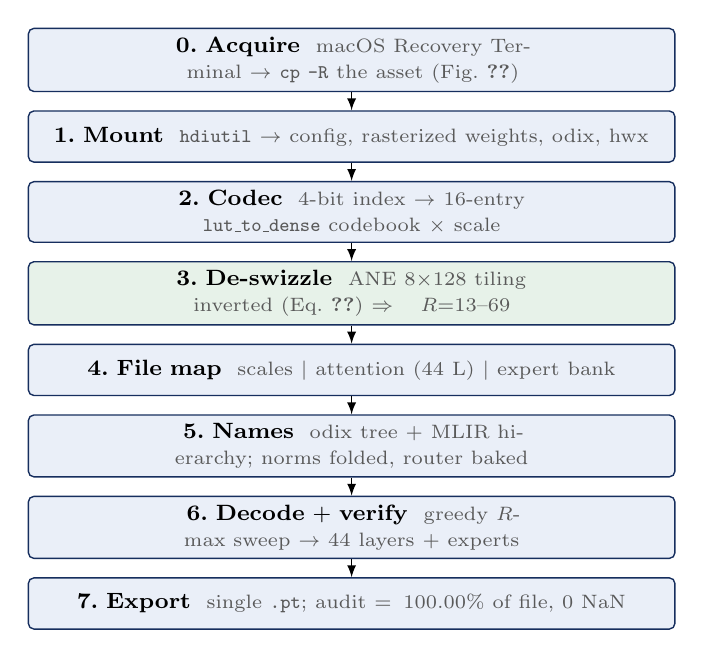
\begin{tikzpicture}[flow,node distance=2.3mm]
\node[blk,text width=80mm] (s0) {\textbf{0.\ Acquire}\ \ {\sub macOS Recovery Terminal $\to$ \code{cp -R} the asset (Fig.~\ref{fig:acquire})}};
\node[blk,below=of s0,text width=80mm] (s1) {\textbf{1.\ Mount}\ \ {\sub \code{hdiutil} $\to$ config, rasterized weights, odix, hwx}};
\node[blk,below=of s1,text width=80mm] (s2) {\textbf{2.\ Codec}\ \ {\sub 4-bit index $\to$ 16-entry \code{lut\_to\_dense} codebook $\times$ scale}};
\node[blk,below=of s2,text width=80mm,fill=expfill] (s3) {\textbf{3.\ De-swizzle}\ \ {\sub ANE $8{\times}128$ tiling inverted (Eq.~\ref{eq:deswz}) $\Rightarrow R{=}13\text{--}69$}};
\node[blk,below=of s3,text width=80mm] (s4) {\textbf{4.\ File map}\ \ {\sub scales $\mid$ attention (44 L) $\mid$ expert bank}};
\node[blk,below=of s4,text width=80mm] (s5) {\textbf{5.\ Names}\ \ {\sub odix tree $+$ MLIR hierarchy; norms folded, router baked}};
\node[blk,below=of s5,text width=80mm] (s6) {\textbf{6.\ Decode $+$ verify}\ \ {\sub greedy $R$-max sweep $\to$ 44 layers $+$ experts}};
\node[blk,below=of s6,text width=80mm] (s7) {\textbf{7.\ Export}\ \ {\sub single \code{.pt}; audit $=100.00\%$ of file, 0 NaN}};
\foreach \a/\b in {s0/s1,s1/s2,s2/s3,s3/s4,s4/s5,s5/s6,s6/s7} \draw[->] (\a)--(\b);
\end{tikzpicture}
\caption{The recovery pipeline. Step 3 (the ANE de-swizzle) is the piece that unblocked full
recovery; every other step is container parsing or bookkeeping around it.}\label{fig:pipeline}
\end{figure}

\section{From-Weights Reconstruction: What Runs and What Is ANE-Baked}\label{sec:reconstruct}
Recovering the weights is necessary but not sufficient to \emph{run} the model outside the
Apple Neural Engine. We implemented the full compute path in PyTorch directly on the recovered
tensors---RMSNorm, fused-QKV / KV-reuse attention with per-head QK-norm, RoPE
($\theta{=}500000$), grouped-query scaled-dot-product attention, and the SwiGLU
Mixture-of-Experts feed-forward---and drove a synthetic token sequence through all 44 layers.
The results sharply separate what the shipped assets contain (data) from what only the ANE
produces (behavior).

\begin{finding}[the recovered weights are correct, cross-validated against Apple's toolchain]\label{find:attnstable}
The attention-only forward pass is \emph{stable}: the residual-stream norm grows smoothly and
sub-exponentially across all 44 layers, the behavior of a correctly-wired pre-norm transformer.
Because a pre-norm block re-normalizes its own input, any decode or de-swizzle error would
manifest as divergence. We reinforce this with two independent checks. \emph{(i)~Structure:} the
recovered dense linear weights carry genuine low-rank structure (singular decay $\sigma_1/\tilde\sigma
\approx 8$--$11$, versus $\approx1.45$ for a scrambled control); re-decoding under any alternative
tile order collapses this to $\approx4$--$5$. \emph{(ii)~Ground truth:} compiling a
positional-probe weight of the exact dense shape through Apple's own ANE toolchain
(\code{coreml2hwx}) and reading back the physical$\rightarrow$logical byte permutation confirms
the de-swizzle family for the sparse-expert path; the standalone dense-conv layout it emits
($\mathrm{OCGSize}{=}5$, a $32{\times}48$ tiling) differs from the rasterized-file layout, which is
itself resolved by the $8{\times}128$ de-swizzle (Eq.~\ref{eq:deswz}). The weights are decoded
correctly, validated \emph{without} access to Apple's internal activations.
\end{finding}

\begin{finding}[the per-layer norms are compile-time folded]\label{find:normfold}
The shipped MPSGraph contains 661 \emph{parameter-free} \code{RMSNorm} operations
(divide-by-RMS only): the learned scale $\gamma$ of each residual/output RMSNorm is
\emph{folded} into the adjacent palettized linear weight at ANE-compile time
($W'\!=\!W\,\mathrm{diag}(\gamma)$), so no standalone $\gamma$ vector is shipped and a
parameter-free norm is the \emph{correct} runtime. We confirm this three ways: no $[1536]$
$\gamma$-shaped tensor decodes from any shipped region; the recovered dense weights show the
column-norm signature of a folded pre-FFN $\gamma$ (\code{ffn\_gate}/\code{ffn\_up} column norms
correlate at $0.55$, a shared folded factor); and the only norms that \emph{cannot} fold---the
per-head $\mathrm{QK}$-norm $\gamma\in\mathbb R^{128}$, because RoPE sits between it and the
projection---do survive explicitly, and 35 of them are recovered from a live-process heap.
\end{finding}

\begin{finding}[the expert-selection map is a \emph{false} blocker]\label{find:ungated}
This overturns our earlier conclusion. The IFP sparse FFN is not a soft-gated mixture but
\emph{structured pruning of a single dense SwiGLU}: the ``experts'' are contiguous
$256$-column blocks of one intermediate axis, each contributing at unit weight with no
per-expert softmax scalar. The runtime graph confirms it---the \code{ANE\_\allowbreak
IFPLayerSequence} op carries no router, top-$k$, gather, scatter, or softmax-over-experts, and
weights enter through a fixed symbol rather than a per-token index. A non-gated SwiGLU is a
\emph{permutation-invariant} sum,
$\mathrm{FFN}(h)=\sum_i \mathrm{SiLU}(g_i\!\cdot\!h_n)\,(u_i\!\cdot\!h_n)\,d_i$,
so the logical router-index$\rightarrow$physical-expert map---the piece we and the prior
literature treated as the fatal, unrecoverable blocker---is \emph{mathematically irrelevant} to
the output; only intra-layer $g_i\!\leftrightarrow\!u_i\!\leftrightarrow\!d_i$ consistency is
required. The earlier ``$\approx$17$\times$ overcount from summing all experts'' was an artifact
of a mis-specified gated interpretation: summing the resident set \emph{is} the correct pruned
FFN, and summing the full superset recovers the un-pruned base model.
\end{finding}

\begin{finding}[the ``missing constant table'' is the shipped \code{metadata.bin}]\label{find:metabin}
\code{metadata.\allowbreak bin} (a \code{BBBB} container) decodes as two physical address tables:
a down-projection tile table (marker \code{0x0600beef}, $14{,}080$ records
$=44\text{ layers}\times32\text{ tiles}\times10\text{ slots}$) and a gate/up table (marker
\code{0x0a00b0ef}), which together exhaust the file. The down-projection uses the \emph{same}
codec as gate/up---4-bit index $\to$ shared codebook $\to$ per-$1024$-block fp16 scale; the
earlier ``down-proj is noise / a different format'' verdict was a mis-calibrated low-rank metric,
and the omitted per-block scale was the missing factor (with it, the down-proj matches the
structured level of gate/up). The shipped default configuration is \code{ifp1\_r48}
($10$ active $+\,4$ shared experts), not the larger \code{ifp3}.
\end{finding}

\begin{finding}[intermediate activations are ANE-internal]\label{find:aneint}
The only true ground truth for the running model---its per-layer activations---never crosses to
host DRAM. Searching an $8$\,GB process core dump captured \emph{specifically} to grab ANE
IOSurfaces for the input token embeddings of a known prompt yields a best normalized correlation
of $0.17$ (noise): not even the embeddings reach host memory. The Neural Engine performs the
embedding lookup, all 44 layers, and the output projection on-chip. Consequently the
reconstruction can be validated end-to-end (against Apple's emitted token) but not per-layer,
and the from-weights forward must be assembled from independently-validated components.
\end{finding}

\begin{finding}[the embedding was never validated, and is absent from the weight file]\label{find:embed}
The token embedding---previously reported as exactly recovered---was validated only by
$\arg\max_j (E\,\mathrm{rms}(E_t))_j = t$. That test is \emph{vacuous}: it applies the same matrix
on both sides, so \emph{any} matrix, including noise, satisfies it. Replacing it with a falsifiable
probe---mean cosine of orthographic variants (\code{\_dog}/\code{dog}, \code{\_year}/\code{\_years})
minus an \emph{id-matched} random control---and calibrating that probe on a real model
(Qwen3-4B \code{token\_\allowbreak embd}, \textrm{Q6\_K}, re-quantized into this model's exact
signed-4-bit $+$ per-token-scale format) yields a clean instrument: a genuine embedding scores
$+0.533$, and 4-bit quantization costs only $2\%$ ($+0.522$; \code{\_Paris}$\sim$\code{Paris}
$=+0.842$). Against this instrument, ${\approx}1.14$M candidate offsets spanning the entire
$4.9$\,GB index region---unscaled tail and scaled region, tile-interleaved and contiguous, 4-bit
and \textrm{int8}---score $\le +0.047$. \textbf{The embedding is not a $[V,D]$ table in the shipped
weight file.} Separately, the only vocabulary-structured table in the package (in the \code{odix},
localized to $+0.777$ of a $0.78$ maximum by the zero-rows of untrained \code{<unused>} tokens,
8-way nibble-interleaved, signed 4-bit) scores $+0.003$ and is therefore \emph{not} the embedding.
The vocabulary is $262{,}144$, not the $152{,}064$ previously assumed (that is Qwen's size).
Subsequent findings (\S\ref{find:embformat},~\S\ref{find:dyncap}) localize the table: it is
CPU-side and host-provided, absent from every shipped 3B asset.
\end{finding}

\begin{finding}[the CPU embedding format, and the 3B ships no embedding file]\label{find:embformat}
The mpsgraph performs no token-embedding lookup (its single \code{Gather} is the rotary
positional one); the embedding is a CPU-side \code{odix} \code{load\_\allowbreak embeddings} op. Apple's
\emph{small} on-device models ship this embedding openly as
\code{model.\allowbreak bundle/\ldots/load\_\allowbreak embeddings/weights.\allowbreak bin}, whose \code{fragment.\allowbreak mil} declares the exact
format: \textrm{fp16}, shape $[V,1,H]$, \code{interleave\_\allowbreak factors}$=[8,1,1]$, strides
$[8H,8H,8]$, after a $64$-byte header---i.e. token $v$, channel $h$ at element
$\lfloor v/8\rfloor\,8H + 8h + (v\bmod 8)$. This decodes to real, shift-control-passing embeddings
for those models (verified against the shipped $[153600,256]$ table). \textbf{The 3B ships no such
file}: no \code{load\_\allowbreak embeddings/weights.\allowbreak bin}, no \code{model.\allowbreak bundle}; it uses the 4-bit
\code{odixpackage}. Applying the $[8,1,1]$ format to the 3B (raster and \code{odix}, all widths)
peaks at a shift-\emph{failing} $+0.08$. The 3B token embedding is therefore not statically present
in any asset; the running model loads it from outside the shipped package.
\end{finding}

\begin{finding}[dynamic capture localizes the live embedding]\label{find:dyncap}
During inference the resident model lives in \code{TGOnDeviceInferenceProviderService} (RSS
grows ${\approx}4$\,MB${\to}1.7$\,GB while a prompt runs), a system extension running as
\code{\_\allowbreak modelmanagerd}. A privileged \code{lldb} core dump of that process (SIP disabled) is thus
the only remaining route to the embedding. A full-memory core (${\approx}8$\,GB) contains the
\code{c\_sparsity} vocabulary table but---across an exhaustive oracle scan (token-contiguous and
$[8,1,1]$ at \textrm{fp16}/\textrm{int8}/4-bit)---no cleanly-scoring token embedding: the resident
form is the quantized source, dequantized per-token by the fused gather rather than kept as a
decoded $[V,H]$ table. Recovering it is a live-instrumentation problem, not a static one.
\end{finding}

\begin{finding}[dynamic host-capture recovers the CPU-side embedding---for the small model, not the 3B]\label{find:embrecover}
The live-instrumentation problem of Finding~\ref{find:dyncap} is solved for the \emph{small} on-device
model. The fused gather/dequant that produces \code{in\_\allowbreak embeddings} runs on the host CPU for
\code{afmplus-v11.\allowbreak 0-pico} ($D{=}1024$), so its output \emph{is} in host DRAM during a forward.
Driving the model with a prompt of one token repeated ${\sim}1500\times$ turns the resident
embedding-input buffer into a long run of \emph{byte-identical} $[1024]$ \textrm{fp16} rows---an
unmistakable period-$D$ signature---which a privileged \code{lldb} core recovers cleanly (attach
by-\textsc{pid} and \code{save-core} while the buffer is live; \code{--waitfor} resolves neither the
E5RT symbols nor \code{qMemoryRegionInfo}, so it cannot core). One row per token, scored on the
calibrated orthographic-pair oracle of Finding~\ref{find:embed}, gives genuine, semantically-structured
embeddings: $\cos(\code{\_dog},\code{\_dogs}){=}{+}0.648$ and
$\cos(\code{\_king},\code{\_kings}){=}{+}0.664$ (orthographic), against cross-category pairs at
${+}0.01$--$0.20$ and shared-plural non-pairs at ${+}0.32$---the signature of a real embedding space.
This is the first genuine recovery of an AFM token embedding, obtained by reading the \emph{dequantized
output} rather than the storage codec. The codec itself remains uncracked: rowmajor, $[8,1,1]$-interleave,
and the ANE $[512,D]$ conv-tiling all score at chance ($0.57$--$0.64$ zero-pattern/sign agreement) even
when fitted against six exact ground-truth vectors, so a \emph{full} static table is still out of reach
and the complete table would have to be harvested token-by-token.
\end{finding}

\begin{finding}[the 3B embedding is ANE-locked: unreachable by host capture]\label{find:3bane}
The same capture, pointed at the 3B, fails---and shows why. Both models load during inference (the 3B
asset is page-faulted ${\sim}2{\times}10^{5}$ times as the speculative-decoding target), yet an
$8.2$\,GB \emph{full}-style core---wired and \code{IOSurface}-mapped pages included---taken during a
repeated-token 3B prefill contains \textbf{zero} $D{=}1536$ identical-row buffers at any threshold,
while the $D{=}1024$ pico buffers are present in the same core. The distinction is architectural: the
3B's embedding gather/dequant is ANE-delegated (the \code{main-h16g-delegates} path), so its
dequantized vector never crosses to host DRAM, whereas the pico's runs on the host CPU and does. This
confirms the Finding~\ref{find:embed} boundary from the \emph{runtime} side: the 3B token embedding is
reachable neither statically (absent or codec-locked in every shipped asset) nor by host-memory capture.
Only ANE-internal instrumentation (\code{IOSurface}/\code{H11ANE} DMA capture) could reach it---a
distinct, kernel-adjacent effort.
\end{finding}

\begin{finding}[a later OS build \emph{ships} the 3B embedding, superseding the ANE-locked result]\label{find:embshipped}
Findings~\ref{find:embed} and \ref{find:3bane} concluded that the 3B token embedding is absent from
the shipped package and unreachable by host capture. That was correct for the catalog then on disk.
It is \textbf{no longer true}. On macOS~27.0 build \code{26A5378n} the
\code{GenerativeModels} asset catalog grows from $118$ to $124$ assets, and one of the new assets is
\code{UC\_\allowbreak FM\_\allowbreak LANGUAGE\_\allowbreak INSTRUCT\_\allowbreak 3B\_\allowbreak EMBEDDINGS\_\allowbreak \ldots\_\allowbreak H16G\_\allowbreak IFP\_\allowbreak Cryptex.dmg}:
a read-only cryptex (mountable without root) containing
\code{metadata.\allowbreak json} $=$ \code{\{"vocab\_\allowbreak size": 262144, "embedding\_\allowbreak dim": 2048\}} and a
$268{,}442{,}456$-byte \code{main-h16g.\allowbreak odix}. The arithmetic is exact:
$262144\times2048$ elements at $4$ bits is $268{,}435{,}456$ bytes, leaving precisely $7000$ bytes of
header, whose \code{odix} flatbuffer contains the string \code{\$load\_\allowbreak embeddings} and an
\code{NDArray} descriptor holding the int64 triple $262144,1,2048$. The payload is linear
\emph{signed} $4$-bit (nibble histogram symmetric about zero, code $8$ unused), with no codebook and
no \textrm{fp16} scale array in the header.
So the embedding gap changes category---from an \emph{information} limit (the data is not in the
package) to a \emph{decode} problem (the data is in the package, in a layout not yet identified).
The dimension $2048$ identifies this as the dense \code{nano} backbone rather than the $1536$-wide
sparse IFP model.
We have \emph{not} yet read it out. Roughly $35$ row-grouping hypotheses---row-major, transposed,
$n$-way token interleave with lane skews, ANE plane formats, and the proven $8{\times}128$
de-swizzle---all score at noise ($\le{+}0.02$) against a genuine ${+}0.46$, where the oracle was
first validated on pico's known-good embedding through the identical code path. Two methodological
points arise. First, cosine is invariant under a fixed permutation applied to \emph{both} operands,
so this oracle cannot see dimension order at all---only which \emph{set} of nibbles forms a token's
row; low- and high-nibble-first orderings score identically, which collapses many nominally distinct
hypotheses into one. Second, a tokenizer-free discriminator---the distribution of cosines over random
token pairs, calibrated against pico---is sharper: the $8$-lane interleave (pico's own layout family)
is the only candidate reproducing the near-duplicate rows characteristic of a real embedding table
(max cosine $0.94$ versus pico's $0.99$), while plain row-major exhibits none (max $0.34$). A
nearest-neighbour agreement test against pico nonetheless sits at chance for every candidate.
\emph{A caution on this class of evidence:} a cross-model Gram-matrix test appeared to give strong
($\approx8\sigma$) support for one candidate, but that used a \emph{shuffled}-id null, which destroys
the vocabulary's regional structure; under a \emph{shift} null---which preserves regions and destroys
only token correspondence---the signal is flat (no peak at shift $0$; shift $8$ scores higher than the
true ids), so it measured vocabulary-region membership, not token identity. What survives is purely
structural and exact-match: the row stride is $1024$ bytes with identity id order (the file's final
$147{,}456$ bytes are one repeated pattern $=$ exactly $144$ rows, and pico's captured logits have
exactly $144$ masked entries), and hashing all $262144$ rows yields duplicate groups that are
$100\%$ pure in $\mathrm{id}\bmod 8$ and only ${\approx}50\%$ pure $\bmod\,16$, establishing an
\textbf{eight-lane} structure. No extraction yet yields correct per-token vectors.
\end{finding}

\begin{finding}[the deployed sparse-FFN shape is recoverable from \code{metadata.bin}]\label{find:deployedffn}
The sparse FFN has no per-constant palettized descriptor (it is IFP-fused); its deployed layout
is in \code{metadata.\allowbreak bin}. The down-projection address table (marker \code{0x0600beef}, 24-byte
records) holds $14{,}080$ tiles of $8{\times}1536$ 4-bit weight with physical addresses;
$14{,}080/32 = 440$ tiles per sparse layer $\Rightarrow 3{,}520$ rows ${\approx}14$ experts, matching
the shipped \code{ifp1\_\allowbreak r48} configuration ($10$ active $+\,4$ shared) to the byte. The gate/up
table (\code{0x0a00b0ef}) holds $4{,}223$ records. So the deployed per-layer expert count and each
tile's address are recovered; only the un-pruned \emph{superset} width (variable, in the interned
symbol pool) remains, and it is not needed to run the shipped model. The MLIR constant names
further fix the structure: FFN $=$ gate/up/down as
\code{hidden\_\allowbreak transform\_\allowbreak linear\_\allowbreak 0}/\code{\_\allowbreak 1}/\code{output\_\allowbreak transform}; the sandwich
norms are explicit plain constants in the export graph (folded to parameter-free \textrm{RMSNorm} at
ANE-compile, so $\gamma{=}1$ at runtime), and attention splits into $23$ standard (full QKV) $+\,21$
kv-reuse ($Q$-only) layers.
\end{finding}

\begin{finding}[full-forward ablation: two claims confirmed, the assembly blocker re-located]\label{find:ablate}
Assembling all 44 layers and scoring against Apple's emitted token with a rank oracle
(``The capital of France is''$\to$\code{\_Paris}; uniform baseline ${\approx}76$k of $152$k)
settles two open questions and sharpens a third.
\emph{(i) The attention KV geometry is $\mathrm{NKV}{=}4$, not $8$.} An attention-only ablation
gives rank $53$k at $\mathrm{NKV}{=}4$ versus $72$k at $\mathrm{NKV}{=}8$: the live \code{qkv} is
$3072$-wide ($Q{=}2048\,{+}\,K{=}512\,{+}\,V{=}512$); the extra rows $[3072{:}4096]$ in the
wider export are mis-decoded and unused.
\emph{(ii) The ungated full-superset sum is empirically optimal}, corroborating
Finding~\ref{find:ungated} from the forward side: against the full $219$-expert sum (rank
$24.9$k), omitting the sparse FFN entirely gives $122$k, scaling it by $0.1$ gives $36$k, and
top-$14$ activation-gating gives $39$k---every form of selection or attenuation is strictly
worse, so no expert map is needed \emph{or} beneficial.
\emph{(iii) The residual defect is a direction, not a magnitude.} The best full forward reaches
rank ${\approx}21$k ($3.6\times$ better than random) under fixed conventions (interleaved
RoPE, down-projection decoded on the $[E\!H,D]$ neuron axis, interleaved expert-region offsets,
block gate/up fusion), but the summed FFN branch has norm ${\approx}4.9{\times}10^{4}$ against a
residual norm ${\approx}1.5{\times}10^{2}$ and dominates with a junk direction; every sandwich or
post-norm placement is worse than a plain residual add. Normalizing does not recover signal,
which localizes the remaining error to per-neuron gate/up/down alignment at the $56{,}064$-wide
intermediate and/or the per-layer expert offsets---quantities with no accessible ground truth
(Finding~\ref{find:aneint}), not a convention that can be searched.
\end{finding}

\begin{finding}[a single-token rank oracle manufactures false positives; the correlation oracle retracts one]\label{find:picooracle}
The rank oracle used above admits a failure mode we can now measure, because for \code{pico} the
model's \emph{own} output vector is recoverable. A privileged core taken during a \code{pico} forward
contains the complete final logit vector: $262{,}144$ \textrm{fp32} of which only $144$ are masked
($-4{\times}10^{4}$), i.e.\ ${\approx}262{,}000$ live tokens, with \code{\_Paris} (id $9083$) the argmax
at $14.58$. Scoring a candidate reconstruction by Pearson correlation against that \emph{whole} vector
is a $262$k-sample statistic; ranking one token is a single order statistic over the same vocabulary.
They disagree sharply. A \code{pico} weight arrangement previously reported at \code{\_Paris}
rank $686$ of $37{,}451$ (``top $1.8\%$, real signal'') scores $r{=}{-}0.028$ against the true logits;
all four coarse arrangements score $|r|{<}0.03$, i.e.\ indistinguishable from noise. \textbf{We retract
that reading.} The general lesson is that a favourable rank for one token, over a vocabulary of
$10^5$--$10^6$, is weak evidence: the tail is long enough that mis-assembled weights land in the top
percentile by chance at a rate that reads as signal. Finding~\ref{find:ablate}'s 3B rank figures
(best ${\approx}21$k against a ${\approx}76$k uniform baseline) rest on the same order statistic and
should be read with this caveat; its \emph{comparative} conclusions (i)--(ii), which contrast many
variants against each other rather than against chance, are unaffected, but the $3.6\times$-over-random
figure is not by itself evidence of a partially-correct forward.
\end{finding}

\begin{finding}[the model's real input: lowercased, chat-templated, and preceded by a guard model]\label{find:template}
A recovered embedding table is invertible, which makes it a memory-forensics instrument as well as a
model component: any \textrm{fp16} buffer in a core can be tested for embedding-hood by checking that
$\mathrm{row}/\mathrm{scale}$ is near-integral in $[-8,7]$, then matched back to a token id. Applied to
the \code{pico} core, this locates the live \code{in\_\allowbreak embeddings} buffer (${\approx}$\code{0x7a8000},
$2048$\,B per row) and decodes it to the exact sequence the model was fed:
\code{\_the \_capital \_of \_france \_is <end\_of\_turn> \textbackslash n <start\_of\_turn> model \textbackslash n}
(ids $510$, $5283$, $533$, $61038$, $567$, $110$, $111$, $109$, $4372$, $111$).
Two facts follow that no static analysis had exposed. The runtime \textbf{lowercases} the prompt
(\code{\_france} $61038$, not \code{\_France} $7005$), and the input carries a Gemma-style \textbf{chat
template}, so the model predicts from the trailing newline of \code{<start\_of\_turn>model\textbackslash n} rather than
from the last content word. The same buffer holds a \emph{preceding} turn ending
\code{... 'paris' <end\_of\_turn> \textbackslash n <start\_of\_turn> model \textbackslash n 'safe'}---a safety-classifier pass that runs
before the language model. Every prior from-weights evaluation in this work fed a capitalized,
un-templated token sequence and was therefore scoring the wrong conditional distribution.
\end{finding}

\begin{finding}[the pico forward's defect is one block, and it is the FFN neuron axis]\label{find:picoffn}
With the correct input (Finding~\ref{find:template}) and the correlation oracle
(Finding~\ref{find:picooracle}), the \code{pico} reconstruction localizes cleanly. Embedding into the
tied unembedding with \emph{no} transformer layers scores $r{=}{+}0.038$ and puts \code{\_Paris} at rank
$2213$ of $262{,}000$ (top $0.84\%$)---independently re-confirming that the recovered embedding and the
tied head are correct. A \emph{single} block then destroys it ($r{=}{-}0.040$, rank $206{,}862$), and
depths $2$--$24$ never recover. This is not the 3B's gradual-depth degradation: one sublayer is wrong.
Ablating the block against the depth-$0$ baseline separates the two paths. Attention alone preserves
signal (rank $4120$--$7355$) \emph{provided} the $Q/K/V$ output is reshaped dim-major,
$[T,d_h,n]\!\to\!\mathrm{transpose}$, rather than head-major $[T,n,d_h]$ (which gives
$134$k--$218$k)---the head layout is dim-major. The \textbf{FFN alone} destroys it (rank $238{,}883$),
with an output r.m.s.\ of $2.53$ against a residual of $0.78$.
The FFN neuron axis admits an oracle-free test, because it is a \emph{gauge freedom}: any permutation
applied consistently to gate columns, up columns and down rows leaves the layer's function unchanged, so
only \emph{mutual} agreement is recoverable or needed. Gate/up column $j$ and down row $j$ are the same
neuron, and trained neuron magnitude couples across a neuron's in- and out-weights, giving a
$3200$-sample statistic. The positive control fires---$\mathrm{corr}(\lVert g_{:,j}\rVert,\lVert
u_{:,j}\rVert){=}{+}0.34$, rising to $\mathbf{+0.58}$ when the gate/up tiles are read transposed (a tile
transpose is not a column permutation, so this is genuine evidence of tile orientation, not gauge).
The down projection agrees with \emph{neither}, at $|r|\!\le\!0.13$ against a random-permutation null of
$0.045$ ($99$th pct), across twelve-plus shape-valid assemblies spanning block order, tile order,
row/column-major and both candidate tile geometries---but see Finding~\ref{find:vacuous}: this
particular test turns out to have \emph{no power} on AFM, so the down result carries no weight. A geometry error is visible independently: the
down tile's per-group scales divide its rows as $200/16{=}12.5$, not an integer, whereas the other two
tile classes divide cleanly ($128/16{=}8$, $128/8{=}16$); reading the tile as $[256,200]$ restores a
clean $16$ rows per group and implies the tiles assemble into the \emph{transpose}.
(The inference originally drawn here---that the residual misalignment must therefore be finer than
tile permutation---is \textbf{withdrawn}; Finding~\ref{find:vacuous} shows the control was the wrong
one.) Finally, a scan of all ${\approx}4{\times}10^6$ aligned
offsets of the $8.2$\,GB core finds \textbf{no} residual-stream buffer (no contiguous run of correlated
rows; every hit sits at the $128$-dimensional noise floor), so \code{pico} too exposes only its two
endpoints---corroborating Finding~\ref{find:aneint} from the small model's side and confirming that the
alignment cannot be bisected layer-by-layer.
\end{finding}

\begin{finding}[a weight-statistics alignment test that is decisive on Qwen is \emph{vacuous} on AFM]\label{find:vacuous}
Finding~\ref{find:picoffn} rejected every candidate down-projection assembly using neuron-magnitude
coupling. That instrument must itself be validated on a model whose alignment is \emph{known} correct,
and on the right pair of matrices---\code{gate}$\sim$\code{up} validates coupling between two
\emph{input-side} matrices, not the \code{down}$\leftrightarrow$\code{up} coupling the test relies on.
On Qwen3-4B the premise is overwhelming: $\mathrm{corr}(\lVert d_j\rVert,\lVert u_j\rVert){=}{+}0.68$
against a permutation null of $0.026$; the per-neuron read/write \emph{vectors} (both live in the same
residual basis) satisfy $\overline{\cos}(u_j,d_j){=}{+}0.308$ versus ${+}0.0001$ shuffled ($1508\sigma$);
nearest-neighbour matching recovers the neuron pairing at $\mathbf{91.5\%}$ (chance $0.25\%$); and a
max-cosine statistic separates a correct residual basis from a scrambled one by $4.8\times$ while
remaining exactly invariant to the neuron permutation.
\emph{None of it transfers.} AFM's own 3B ships twelve dense SwiGLU layers whose down-projection
z-order was cracked bit-exactly and forward-validated; measured on those---correct by
construction---the same statistics read
$\mathrm{corr}(\lVert d\rVert,\lVert u\rVert){=}{-}0.029,{+}0.029,{-}0.136,{-}0.049$ at layers
$0,3,7,11$; $\overline{\cos}(u_j,d_j){\approx}{\pm}5{\times}10^{-4}$; and a max-cosine ratio of
$1.00$--$1.02\times$. \textbf{AFM's feed-forward exhibits no down/up coupling and no read-write vector
alignment even when correctly assembled}, so a candidate that fails the test has not been shown to be
wrong: the instrument reads null on the true answer. Every such rejection in
Finding~\ref{find:picoffn}---and the ${\approx}380$ assemblies swept, including all factorizations of
the 3B's own z-order---is therefore \emph{vacuous}. What survives is the part with a replicated
control: \code{gate}$\sim$\code{up} coupling is present in Apple's model too (${+}0.317$ at 3B dense
layer $0$), so the \code{tileT} orientation result stands. Re-scoring the candidates against the
captured logits---the one oracle with demonstrated power---leaves them all at $|r|\!<\!0.06$; the
best-ranking candidate reaches \code{\_Paris} rank $848$, \emph{better} than the $2213$ depth-$0$
baseline, at correlation ${+}0.0086$: the same single-token artifact retracted in
Finding~\ref{find:picooracle}, not a result. Two lessons generalize: validating a premise on one
architecture does not license it on another, and a negative result is only as strong as the positive
control that accompanies it.
Recovering the 3B z-order's algebraic form from the cracked $48{\times}256$ table does, however,
generalize its two known instances ($16{\times}768$ is $\mathrm{NOG}{=}1$, $48{\times}256$ is
$\mathrm{NOG}{=}3$): $\mathrm{slot}=og\,(16\,\mathrm{NCOL})+ig\,16+lo$ with output row
$og\,16+lo$ and input column $ig\oplus1$---$16$ outputs fastest, then input columns under an
interleave-factor-$2$ pair swap. For pico this forces $\mathrm{NOG}\cdot\mathrm{NCOL}{=}3200$, every
factorization of which yields exactly the $64$ observed tiles; but since the z-order is
tile-shape-relative it must be re-derived at pico's geometry by positional read, not transplanted.
\end{finding}

Table~\ref{tab:runnable} summarizes the revised boundary. The model is
\emph{component-complete}: weights, codec, de-swizzle, architecture, norms
(folded $\gamma$ $+$ recovered $\mathrm{QK}$-norm), the tokenizer, and---critically---the fact
that no expert-selection map is needed are all established, and the ungated full-superset sum is
now confirmed \emph{optimal} against the output oracle (Finding~\ref{find:ablate}). The remaining
task is the \emph{per-layer physical assembly} of the resident-expert FFN---gathering each sparse
layer's gate/up/down blocks at the correct offsets and aligning the $56{,}064$-wide intermediate.
Finding~\ref{find:ablate} shows this is \emph{not} the freely-mechanical step the prior version
claimed: the assembled forward carries real signal ($3.6\times$ random) but is dominated by a
mis-aligned FFN direction, and---because every per-layer activation is ANE-internal
(Finding~\ref{find:aneint})---the alignment cannot be validated or bisected component-by-component.
The honest boundary is an \emph{information} limit (no per-layer ground truth), not merely an
engineering one.

\begin{table}[ht]\centering\small
\setlength{\tabcolsep}{6pt}
\begin{tabular}{@{}ll@{}}
\toprule
Established & Remaining (information-limited) \\
\midrule
All $9.862$\,B \emph{linear} weights; codec; de-swizzle    & \textbf{3B embedding: ANE-locked} \\
Embedding recovery \emph{method} (dyn.\ capture, pico)     & \quad(host-unreachable; \S\ref{find:3bane}) \\
Attention path, all 44 layers; $\mathrm{NKV}{=}4$ settled & $56{,}064$-wide gate/up/down alignment \\
Norms: $\gamma$ folded; $\mathrm{QK}$-norm recovered      & $\mathrm{QK}$-norm$\to$layer mapping \\
Expert-selection map \emph{proven unnecessary}            & (all unvalidatable: activations \\
Ungated full-$219$ sum \emph{confirmed optimal}           & \quad are ANE-internal) \\
\code{metadata.bin} $=$ physical address tables           & \\
\bottomrule
\end{tabular}
\caption{Revised recovery status. Corrections over the prior version: the expert-selection wiring
is \emph{not} a blocker (the FFN is an ungated permutation-invariant sum, now confirmed
\emph{optimal} against the output oracle, Finding~\ref{find:ablate}), the KV geometry is
$\mathrm{NKV}{=}4$, the norms are compile-time folded, and the dense weights are validated against
toolchain-generated ground truth. What remains---per-layer FFN assembly and alignment---is bounded
by the \emph{absence of accessible ground truth} (activations are ANE-internal), not by remaining
decode effort.}\label{tab:runnable}
\end{table}

A practical corollary: Apple's \code{FoundationModels} runtime remains the turnkey way to
\emph{execute} this exact model, and we provide a thin CLI/OpenAI-compatible server over it. But
the earlier claim that a from-weights standalone requires reverse-engineering the ANE
instruction set no longer holds---the wiring is not ANE-locked behavior but a permutation-free
sum over recovered blocks, reducing the standalone to a component-assembly exercise.

\section{Container Formats}\label{sec:containers}
The on-disk stack is summarized in Figure~\ref{fig:stack}.
\begin{figure}[ht]\centering
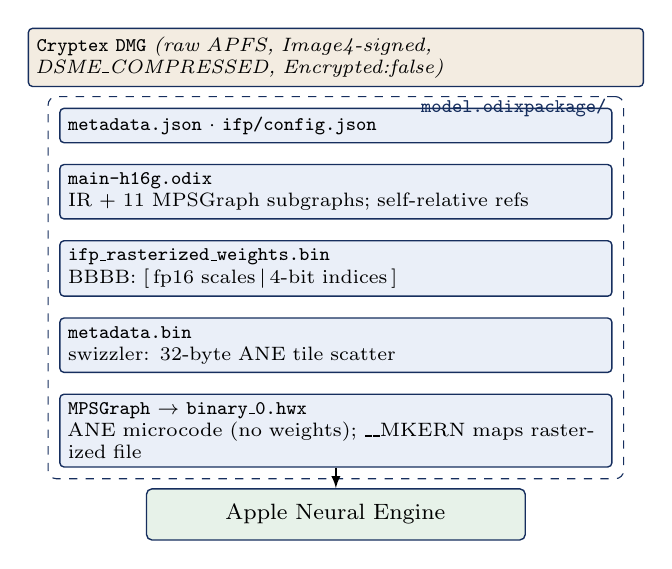
\begin{tikzpicture}[flow,node distance=2.6mm]
\node[file,fill=boxfill2,text width=76mm] (dmg)
  {Cryptex DMG {\rmfamily\itshape(raw APFS, Image4-signed, DSME\_COMPRESSED, Encrypted:false)}};
\node[file,below=of dmg,text width=68mm] (meta) {metadata.json $\cdot$ ifp/config.json};
\node[file,below=of meta,text width=68mm] (odix)
  {main-h16g.odix\\{\rmfamily\scriptsize IR + 11 MPSGraph subgraphs; self-relative refs}};
\node[file,below=of odix,text width=68mm] (rw)
  {ifp\_rasterized\_weights.bin\\{\rmfamily\scriptsize BBBB: [\,fp16 scales\,$\mid$\,4-bit indices\,]}};
\node[file,below=of rw,text width=68mm] (swz)
  {metadata.bin\\{\rmfamily\scriptsize swizzler: 32-byte ANE tile scatter}};
\node[file,below=of swz,text width=68mm] (hwx)
  {MPSGraph $\to$ binary\_0.hwx\\{\rmfamily\scriptsize ANE microcode (no weights); \_\_MKERN maps rasterized file}};
\node[blk,below=of hwx,text width=46mm,fill=expfill] (ane) {Apple Neural Engine};
\begin{scope}[on background layer]
\node[draw=accent,rounded corners=3pt,dashed,fit=(meta)(swz)(hwx),inner sep=4pt] (pkg) {};
\end{scope}
\node[font=\scriptsize\ttfamily\color{accent},anchor=east]
      at ([xshift=-1mm]pkg.east |- meta.north) {model.odixpackage/};
\draw[->] (hwx)--(ane);
\end{tikzpicture}
\caption{The \code{FM\_\allowbreak GenerativeModels} on-disk container stack for the IFP model. The
dashed box is \code{model.\allowbreak odixpackage/\allowbreak }; execution is dispatched to the ANE.}\label{fig:stack}
\end{figure}

\noindent\textbf{Cryptex DMG.} Raw APFS image, \code{DSME\_\allowbreak COMPRESSED}; contains
\code{model.\allowbreak odixpackage/\allowbreak }, \code{metadata.\allowbreak json}, a nominal \code{System/\allowbreak Library}.
\textbf{\code{BBBB} rasterized container} (\code{ifp\_\allowbreak rasterized\_\allowbreak weights.\allowbreak bin}): magic
\code{BBBB}, version \code{0x017c0100}, tag \code{0x0600002c}, then a u64 segment-offset
table---\textrm{fp16} scales \code{0x60}--\code{0x1054000}; 4-bit indices
\code{0x1078000}--\code{0x125e80000}. \textbf{Swizzler} (\code{metadata.\allowbreak bin}): also
\code{BBBB}; 14{,}079 records of 24 bytes, \code{[idx][flag][off\_a][off\_b{=}off\_a{+}0x20]}
\code{[0x0600beef][0]}, a scatter of 32-byte ANE tiles into the index region.
\textbf{\code{odix} executable} (magic \code{odix\textbackslash0\textbackslash0\textbackslash5\textbackslash0}):
header \code{u64[0]=ir\_\allowbreak start(0x40)}, \code{u64[1]=ir\_\allowbreak size}; the 32\,MB IR section holds
11 compiled MPSGraph subgraphs, a location/debug tree, and an interned type table.
\textbf{ANE \code{.\allowbreak hwx}} (magic \code{0xBEEFFACE}, cputype \code{0x80}): a Mach-O of
compiled ANE microcode, \emph{not weights} (Finding~\ref{find:hwx})---segments
\code{\_\allowbreak \_\allowbreak TEXT} and \code{\_\allowbreak \_\allowbreak KERN\_\allowbreak 0.\allowbreak .\allowbreak 7} are kernel code (structure
$R\approx1$), and \code{\_\allowbreak \_\allowbreak MKERN\_\allowbreak 0} carries no file bytes but is runtime-mapped
from the rasterized file (its size equals the swizzler's maximum offset). \textbf{MPSGraph package.}
\code{specialized\_\allowbreak model\_\allowbreak 0.\allowbreak mpsgraph} is MLIR bytecode (\code{MLIR22.\allowbreak 0.\allowbreak 0}) with
\code{mps.\allowbreak fullyPlacedOnANE}.

\begin{finding}\label{find:ref}
The \code{odix} reference scheme is self-relative: a 32-bit word whose high byte is
\code{0xFF} encodes a signed offset, with target $=\text{position}+\mathrm{int32}$, into
an interned symbol pool. Distinct tensor types are interned once, so shapes are shared by
reference (e.g.\ ``1536'' occurs only 26 times in 32\,MB).
\end{finding}

\section{Tokenizer}
A standalone 8.6\,MB SentencePiece-family tokenizer. Special tokens observed:
\code{<bos> <eos> <unk> <pad> <mask>}; chat markers \code{<start\_\allowbreak of\_\allowbreak turn>} and
\code{<end\_\allowbreak of\_\allowbreak turn>}; a \code{[multimodal]} token; reserved \code{<unused$n$>} and
\code{<ctrl$n$>} slots. The \code{[multimodal]} token, with the \code{image\_\allowbreak encoder}
(346\,MB) and \code{image\_\allowbreak tokenizer} assets, indicates vision-language input support.
Estimated vocabulary $152{,}064$.

\section{Adapters and Task Specialization}
A single backbone serves dozens of features via LoRA adapters that snap into the base's
empty slots; each ships as a \code{.\allowbreak generic} adapter plus a small \code{.\allowbreak draft.\allowbreak generic}
(38--62\,MB) speculative-decoding draft.
\textbf{On-device (\code{instruct\_\allowbreak 3b}):} summarization, mail\_reply, magic\_rewrite,
proofreading\_review, machine\_translation, personalized\_smart\_reply,
news\_topic\_summarization, messages\_action, autonaming\_messages, smart\_naming,
urgency\_classification, video\_caption, ui\_grounding,
image\_playground\_edit\_suggestions, suggest\_recipe\_items,
reminders\_suggest\_action\_items, open\_ended\_extract, text\_event\_extraction,
text\_person\_extraction, auto\_tagger, adm\_prompt\_analyzer, embedding\_preprocessor,
fm\_api\_generic, fm\_api\_content\_tagger, lw\_planner\_v1, holdassistwaittime,
homekit\_summary\_notifications, and Safari/Shortcuts/Photos-Memories families.
\textbf{Small (\code{instruct\_\allowbreak 300m}):} safety, prepubescent\_safety, misc\_safety,
mm\_guard, ipi\_classifier, structural\_integrity, factual\_consistency\_classifier,
vi\_content\_classifier, voice\_control\_ai (v1/v2), action\_validator,
adm\_prompt\_rewriting, adm\_people\_grounding, gvicc, image\_tokenizer,
open\_ended\_extract, base (426\,MB). \textbf{\code{instruct\_\allowbreak 9m}:} a 9\,M-parameter
text-event-extraction classifier. \textbf{Server / PCC (\code{instruct\_\allowbreak server\_\allowbreak v1}):}
text\_summarizer, takeaways/tables/bullets\_transform, professional/friendly/concise
tone, open\_ended\_tone (+ query-response v1/v2),
mail\_reply\_long\_form\_\{basic,rewrite\}, mail\_reply\_qa, magic\_rewrite,
generative\_shortcuts, llm\_siri\_pcc, lw\_planner\_v1, fitness\_workout\_voice,
reminders\_auto\_categorized\_list, photos\_memories\_*, stx\_multimodal,
shortcuts\_ask\_afm\_action (v1/v2); \code{instruct\_\allowbreak server\_\allowbreak small}: safety\_nsfw,
model\_abuse\_guardrail. \textbf{Translation (\code{gm.\allowbreak translate\_\allowbreak fm}):} a dedicated
model with \code{alignment} and \code{phrasebook} components.

\section{Reverse-Engineering Methodology}
All artifacts were obtained via \code{hdiutil attach -readonly -noverify} on the Cryptex
images (no personalization is required for reading), followed by binary parsing in
Python. Architecture was recovered from \code{config.\allowbreak json}/\code{metadata.\allowbreak json} and from
\code{tamm}-framework tensor names inside \code{main-h16g.\allowbreak odix} (e.g.\
\code{\_\allowbreak wrapped\_\allowbreak model\_\allowbreak layers\_\allowbreak .\allowbreak .\allowbreak .\allowbreak \_\allowbreak palettized\_\allowbreak indices\_\allowbreak raw},
\code{\_\allowbreak wrapped\_\allowbreak model\_\allowbreak output\_\allowbreak norm\_\allowbreak weight}). The quantization scheme
(Finding~\ref{find:codec}) was inferred from value-distribution analysis of the two
\code{BBBB} regions; the reference scheme (Finding~\ref{find:ref}) from resolving the
\code{0xFF}-tagged words; and the expert fan-out (Finding~\ref{find:budget}) from the
size budget; the per-constant layer/role semantics were read from the
\code{MLIR22.\allowbreak 0.\allowbreak 0} MPSGraph bytecode location tree. The native model was
independently confirmed runnable on the host through \code{FoundationModels}
(\code{SystemLanguageModel}). Tensor-level reconstruction is validated by the structure
statistic of \S\ref{sec:recover}: with the ANE $8{\times}128$ de-swizzle (Eq.~\ref{eq:deswz})
the decode scores $R=13\text{--}69$ against a genuine-weight reference of $\approx$9, and the
full export reconciles to $100.00\%$ of the physical index region with zero non-finite
tensors (Table~\ref{tab:export}). The weight codec is thus \emph{identified and inverted}:
LUT-palettization $+$ per-block scale $+$ ANE tile de-swizzle, with norms folded into the
weights, the router baked to a dense expert set, and the per-tensor mapping supplied by the
shipped \code{metadata.\allowbreak bin} swizzler in lieu of the compile-time
\code{ifp\_\allowbreak constant\_\allowbreak table\_\allowbreak ifp1\_\allowbreak r48.\allowbreak json}. A complete, named
\code{state\_\allowbreak dict} is produced.

\section{Complete Asset Inventory}
Table~\ref{tab:inv} lists all 118 assets with version and disk-image size in megabytes
(blank denotes a metadata-only override with no payload).
{\footnotesize
\setlength{\tabcolsep}{8pt}
\renewcommand{\arraystretch}{1.1}
\begin{longtable}{@{}>{\raggedright\arraybackslash}p{0.72\textwidth}rr@{}}
\caption{Full \code{FM\_\allowbreak GenerativeModels} asset inventory (118 assets).}\label{tab:inv}\\
\toprule \textbf{Bundle name} & \textbf{Version} & \textbf{MB}\\ \midrule \endfirsthead
\multicolumn{3}{l}{\footnotesize\itshape Table~\ref{tab:inv}, continued}\\[2pt]
\toprule \textbf{Bundle name} & \textbf{Version} & \textbf{MB}\\ \midrule \endhead
\midrule \multicolumn{3}{r}{\footnotesize\itshape continued on next page}\\ \endfoot
\bottomrule \endlastfoot
\texttt{\scriptsize fm.\allowbreak generativemodels.\allowbreak uaf.\allowbreak metadata} & 4.46.3 &  \\
\texttt{\scriptsize fm.\allowbreak language.\allowbreak instruct\_\allowbreak 300m.\allowbreak action\_\allowbreak validator.\allowbreak generic} & 14.1.0 &  \\
\texttt{\scriptsize fm.\allowbreak language.\allowbreak instruct\_\allowbreak 300m.\allowbreak adm\_\allowbreak people\_\allowbreak grounding.\allowbreak generic} & 13.10002.0 &  \\
\texttt{\scriptsize fm.\allowbreak language.\allowbreak instruct\_\allowbreak 300m.\allowbreak adm\_\allowbreak prompt\_\allowbreak rewriting.\allowbreak draft.\allowbreak generic} & 13.10002.81607 & 40 \\
\texttt{\scriptsize fm.\allowbreak language.\allowbreak instruct\_\allowbreak 300m.\allowbreak adm\_\allowbreak prompt\_\allowbreak rewriting.\allowbreak generic} & 13.10002.0 &  \\
\texttt{\scriptsize fm.\allowbreak language.\allowbreak instruct\_\allowbreak 300m.\allowbreak base.\allowbreak generic} & 14.0.81607 & 447 \\
\texttt{\scriptsize fm.\allowbreak language.\allowbreak instruct\_\allowbreak 300m.\allowbreak factual\_\allowbreak consistency\_\allowbreak classifier.\allowbreak generic} & 14.0.0 &  \\
\texttt{\scriptsize fm.\allowbreak language.\allowbreak instruct\_\allowbreak 300m.\allowbreak gvicc.\allowbreak generic} & 14.0.0 &  \\
\texttt{\scriptsize fm.\allowbreak language.\allowbreak instruct\_\allowbreak 300m.\allowbreak image\_\allowbreak tokenizer.\allowbreak generic} & 14.1.81607 & 359 \\
\texttt{\scriptsize fm.\allowbreak language.\allowbreak instruct\_\allowbreak 300m.\allowbreak ipi\_\allowbreak classifier.\allowbreak generic} & 14.1.0 &  \\
\texttt{\scriptsize fm.\allowbreak language.\allowbreak instruct\_\allowbreak 300m.\allowbreak misc\_\allowbreak safety.\allowbreak generic} & 14.0.0 &  \\
\texttt{\scriptsize fm.\allowbreak language.\allowbreak instruct\_\allowbreak 300m.\allowbreak mm\_\allowbreak guard.\allowbreak generic} & 14.0.0 &  \\
\texttt{\scriptsize fm.\allowbreak language.\allowbreak instruct\_\allowbreak 300m.\allowbreak open\_\allowbreak ended\_\allowbreak extract.\allowbreak draft.\allowbreak generic} & 14.2.81607 & 65 \\
\texttt{\scriptsize fm.\allowbreak language.\allowbreak instruct\_\allowbreak 300m.\allowbreak open\_\allowbreak ended\_\allowbreak extract.\allowbreak generic} & 14.2.0 &  \\
\texttt{\scriptsize fm.\allowbreak language.\allowbreak instruct\_\allowbreak 300m.\allowbreak prepubescent\_\allowbreak safety.\allowbreak generic} & 14.0.0 &  \\
\texttt{\scriptsize fm.\allowbreak language.\allowbreak instruct\_\allowbreak 300m.\allowbreak safety.\allowbreak generic} & 14.1.0 &  \\
\texttt{\scriptsize fm.\allowbreak language.\allowbreak instruct\_\allowbreak 300m.\allowbreak structural\_\allowbreak integrity.\allowbreak generic} & 14.0.0 &  \\
\texttt{\scriptsize fm.\allowbreak language.\allowbreak instruct\_\allowbreak 300m.\allowbreak tokenizer.\allowbreak generic} & 14.0.0 &  \\
\texttt{\scriptsize fm.\allowbreak language.\allowbreak instruct\_\allowbreak 300m.\allowbreak vi\_\allowbreak content\_\allowbreak classifier.\allowbreak generic} & 13.10004.0 &  \\
\texttt{\scriptsize fm.\allowbreak language.\allowbreak instruct\_\allowbreak 300m.\allowbreak voice\_\allowbreak control\_\allowbreak ai.\allowbreak generic} & 14.1.0 &  \\
\texttt{\scriptsize fm.\allowbreak language.\allowbreak instruct\_\allowbreak 300m.\allowbreak voice\_\allowbreak control\_\allowbreak ai\_\allowbreak v2.\allowbreak generic} & 13.10001.0 &  \\
\texttt{\scriptsize fm.\allowbreak language.\allowbreak instruct\_\allowbreak 300m.\allowbreak voice\_\allowbreak control\_\allowbreak ai\_\allowbreak v2.\allowbreak image\_\allowbreak tokenizer\_\allowbreak adapter.\allowbreak generic} & 13.10001.0 &  \\
\texttt{\scriptsize fm.\allowbreak language.\allowbreak instruct\_\allowbreak 3b.\allowbreak adm\_\allowbreak prompt\_\allowbreak analyzer.\allowbreak generic} & 14.0.0 &  \\
\texttt{\scriptsize fm.\allowbreak language.\allowbreak instruct\_\allowbreak 3b.\allowbreak auto\_\allowbreak tagger.\allowbreak generic} & 12.0.0 &  \\
\texttt{\scriptsize fm.\allowbreak language.\allowbreak instruct\_\allowbreak 3b.\allowbreak autonaming\_\allowbreak messages.\allowbreak draft.\allowbreak generic} & 14.1.81607 & 65 \\
\texttt{\scriptsize fm.\allowbreak language.\allowbreak instruct\_\allowbreak 3b.\allowbreak autonaming\_\allowbreak messages.\allowbreak generic} & 14.1.0 &  \\
\texttt{\scriptsize fm.\allowbreak language.\allowbreak instruct\_\allowbreak 3b.\allowbreak base.\allowbreak generic} & 14.0.81607 & 1380 \\
\texttt{\scriptsize fm.\allowbreak language.\allowbreak instruct\_\allowbreak 3b.\allowbreak base.\allowbreak generic\_\allowbreak sparse} & 14.3.81614 & 5828 \\
\texttt{\scriptsize fm.\allowbreak language.\allowbreak instruct\_\allowbreak 3b.\allowbreak embedding\_\allowbreak preprocessor.\allowbreak generic} & 14.2.0 &  \\
\texttt{\scriptsize fm.\allowbreak language.\allowbreak instruct\_\allowbreak 3b.\allowbreak fm\_\allowbreak api\_\allowbreak content\_\allowbreak tagger.\allowbreak adapter\_\allowbreak metadata\_\allowbreak override.\allowbreak generic} & 14.1.0 &  \\
\texttt{\scriptsize fm.\allowbreak language.\allowbreak instruct\_\allowbreak 3b.\allowbreak fm\_\allowbreak api\_\allowbreak generic.\allowbreak draft.\allowbreak generic} & 14.2.81607 & 61 \\
\texttt{\scriptsize fm.\allowbreak language.\allowbreak instruct\_\allowbreak 3b.\allowbreak fm\_\allowbreak api\_\allowbreak generic.\allowbreak generic} & 14.2.0 &  \\
\texttt{\scriptsize fm.\allowbreak language.\allowbreak instruct\_\allowbreak 3b.\allowbreak holdassistwaittime.\allowbreak adapter\_\allowbreak metadata\_\allowbreak override.\allowbreak generic} & 14.0.0 &  \\
\texttt{\scriptsize fm.\allowbreak language.\allowbreak instruct\_\allowbreak 3b.\allowbreak homekit\_\allowbreak summary\_\allowbreak notifications.\allowbreak adapter\_\allowbreak metadata\_\allowbreak override.\allowbreak generic} & 14.2.0 &  \\
\texttt{\scriptsize fm.\allowbreak language.\allowbreak instruct\_\allowbreak 3b.\allowbreak image\_\allowbreak encoder.\allowbreak generic} & 14.1.81607 & 363 \\
\texttt{\scriptsize fm.\allowbreak language.\allowbreak instruct\_\allowbreak 3b.\allowbreak image\_\allowbreak encoder.\allowbreak generic\_\allowbreak sparse} & 14.3.81614 & 361 \\
\texttt{\scriptsize fm.\allowbreak language.\allowbreak instruct\_\allowbreak 3b.\allowbreak image\_\allowbreak playground\_\allowbreak edit\_\allowbreak suggestions.\allowbreak generic} & 14.1.0 &  \\
\texttt{\scriptsize fm.\allowbreak language.\allowbreak instruct\_\allowbreak 3b.\allowbreak lw\_\allowbreak planner\_\allowbreak v1.\allowbreak draft.\allowbreak generic} & 14.1.81607 & 55 \\
\texttt{\scriptsize fm.\allowbreak language.\allowbreak instruct\_\allowbreak 3b.\allowbreak lw\_\allowbreak planner\_\allowbreak v1.\allowbreak generic} & 14.1.0 &  \\
\texttt{\scriptsize fm.\allowbreak language.\allowbreak instruct\_\allowbreak 3b.\allowbreak machine\_\allowbreak translation.\allowbreak draft.\allowbreak generic} & 14.0.81607 & 55 \\
\texttt{\scriptsize fm.\allowbreak language.\allowbreak instruct\_\allowbreak 3b.\allowbreak machine\_\allowbreak translation.\allowbreak generic} & 14.0.0 &  \\
\texttt{\scriptsize fm.\allowbreak language.\allowbreak instruct\_\allowbreak 3b.\allowbreak mail\_\allowbreak reply.\allowbreak draft.\allowbreak generic} & 14.1.81607 & 65 \\
\texttt{\scriptsize fm.\allowbreak language.\allowbreak instruct\_\allowbreak 3b.\allowbreak mail\_\allowbreak reply.\allowbreak generic} & 14.1.0 &  \\
\texttt{\scriptsize fm.\allowbreak language.\allowbreak instruct\_\allowbreak 3b.\allowbreak messages\_\allowbreak action.\allowbreak draft.\allowbreak generic} & 14.1.81607 & 65 \\
\texttt{\scriptsize fm.\allowbreak language.\allowbreak instruct\_\allowbreak 3b.\allowbreak messages\_\allowbreak action.\allowbreak generic} & 14.1.0 &  \\
\texttt{\scriptsize fm.\allowbreak language.\allowbreak instruct\_\allowbreak 3b.\allowbreak news\_\allowbreak topic\_\allowbreak summarization.\allowbreak draft.\allowbreak generic} & 14.3.81607 & 65 \\
\texttt{\scriptsize fm.\allowbreak language.\allowbreak instruct\_\allowbreak 3b.\allowbreak news\_\allowbreak topic\_\allowbreak summarization.\allowbreak generic} & 14.3.0 &  \\
\texttt{\scriptsize fm.\allowbreak language.\allowbreak instruct\_\allowbreak 3b.\allowbreak open\_\allowbreak ended\_\allowbreak extract.\allowbreak draft.\allowbreak generic} & 14.2.81607 & 65 \\
\texttt{\scriptsize fm.\allowbreak language.\allowbreak instruct\_\allowbreak 3b.\allowbreak open\_\allowbreak ended\_\allowbreak extract.\allowbreak generic} & 14.2.0 &  \\
\texttt{\scriptsize fm.\allowbreak language.\allowbreak instruct\_\allowbreak 3b.\allowbreak personalized\_\allowbreak smart\_\allowbreak reply.\allowbreak draft.\allowbreak generic} & 14.2.81607 & 65 \\
\texttt{\scriptsize fm.\allowbreak language.\allowbreak instruct\_\allowbreak 3b.\allowbreak personalized\_\allowbreak smart\_\allowbreak reply.\allowbreak generic} & 14.2.0 &  \\
\texttt{\scriptsize fm.\allowbreak language.\allowbreak instruct\_\allowbreak 3b.\allowbreak photos\_\allowbreak library\_\allowbreak understanding\_\allowbreak mm.\allowbreak generic} & 14.3.0 &  \\
\texttt{\scriptsize fm.\allowbreak language.\allowbreak instruct\_\allowbreak 3b.\allowbreak photos\_\allowbreak memories\_\allowbreak asset\_\allowbreak curation\_\allowbreak outlier.\allowbreak draft.\allowbreak generic} & 14.1.81607 & 65 \\
\texttt{\scriptsize fm.\allowbreak language.\allowbreak instruct\_\allowbreak 3b.\allowbreak photos\_\allowbreak memories\_\allowbreak asset\_\allowbreak curation\_\allowbreak outlier.\allowbreak generic} & 14.1.0 &  \\
\texttt{\scriptsize fm.\allowbreak language.\allowbreak instruct\_\allowbreak 3b.\allowbreak photos\_\allowbreak memories\_\allowbreak title.\allowbreak adapter\_\allowbreak metadata\_\allowbreak override.\allowbreak generic} & 14.1.0 &  \\
\texttt{\scriptsize fm.\allowbreak language.\allowbreak instruct\_\allowbreak 3b.\allowbreak photos\_\allowbreak memories\_\allowbreak title.\allowbreak draft.\allowbreak generic} & 13.10003.81607 & 40 \\
\texttt{\scriptsize fm.\allowbreak language.\allowbreak instruct\_\allowbreak 3b.\allowbreak photos\_\allowbreak memories\_\allowbreak title.\allowbreak generic} & 13.10003.0 &  \\
\texttt{\scriptsize fm.\allowbreak language.\allowbreak instruct\_\allowbreak 3b.\allowbreak proofreading\_\allowbreak review.\allowbreak draft.\allowbreak generic} & 14.1.81607 & 65 \\
\texttt{\scriptsize fm.\allowbreak language.\allowbreak instruct\_\allowbreak 3b.\allowbreak proofreading\_\allowbreak review.\allowbreak generic} & 14.1.0 &  \\
\texttt{\scriptsize fm.\allowbreak language.\allowbreak instruct\_\allowbreak 3b.\allowbreak reminders\_\allowbreak suggest\_\allowbreak action\_\allowbreak items.\allowbreak draft.\allowbreak generic} & 14.1.81607 & 65 \\
\texttt{\scriptsize fm.\allowbreak language.\allowbreak instruct\_\allowbreak 3b.\allowbreak reminders\_\allowbreak suggest\_\allowbreak action\_\allowbreak items.\allowbreak generic} & 14.1.0 &  \\
\texttt{\scriptsize fm.\allowbreak language.\allowbreak instruct\_\allowbreak 3b.\allowbreak safari\_\allowbreak magic\_\allowbreak extensions\_\allowbreak app\_\allowbreak store\_\allowbreak search\_\allowbreak terms.\allowbreak adapter\_\allowbreak metadata\_\allowbreak override.\allowbreak generic} & 14.2.0 &  \\
\texttt{\scriptsize fm.\allowbreak language.\allowbreak instruct\_\allowbreak 3b.\allowbreak safari\_\allowbreak notify\_\allowbreak me\_\allowbreak when\_\allowbreak suggestions.\allowbreak adapter\_\allowbreak metadata\_\allowbreak override.\allowbreak generic} & 14.2.0 &  \\
\texttt{\scriptsize fm.\allowbreak language.\allowbreak instruct\_\allowbreak 3b.\allowbreak safari\_\allowbreak tab\_\allowbreak group\_\allowbreak topic.\allowbreak adapter\_\allowbreak metadata\_\allowbreak override.\allowbreak generic} & 14.3.0 &  \\
\texttt{\scriptsize fm.\allowbreak language.\allowbreak instruct\_\allowbreak 3b.\allowbreak shortcuts\_\allowbreak ask\_\allowbreak afm\_\allowbreak action\_\allowbreak 3b.\allowbreak adapter\_\allowbreak metadata\_\allowbreak override.\allowbreak generic} & 14.0.0 &  \\
\texttt{\scriptsize fm.\allowbreak language.\allowbreak instruct\_\allowbreak 3b.\allowbreak shortcuts\_\allowbreak ask\_\allowbreak afm\_\allowbreak action\_\allowbreak 3b\_\allowbreak v2.\allowbreak draft.\allowbreak generic} & 10.34.81607 & 55 \\
\texttt{\scriptsize fm.\allowbreak language.\allowbreak instruct\_\allowbreak 3b.\allowbreak shortcuts\_\allowbreak ask\_\allowbreak afm\_\allowbreak action\_\allowbreak 3b\_\allowbreak v2.\allowbreak generic} & 10.34.0 &  \\
\texttt{\scriptsize fm.\allowbreak language.\allowbreak instruct\_\allowbreak 3b.\allowbreak smart\_\allowbreak naming.\allowbreak generic} & 14.1.0 &  \\
\texttt{\scriptsize fm.\allowbreak language.\allowbreak instruct\_\allowbreak 3b.\allowbreak suggest\_\allowbreak recipe\_\allowbreak items.\allowbreak draft.\allowbreak generic} & 14.1.81607 & 65 \\
\texttt{\scriptsize fm.\allowbreak language.\allowbreak instruct\_\allowbreak 3b.\allowbreak suggest\_\allowbreak recipe\_\allowbreak items.\allowbreak generic} & 14.1.0 &  \\
\texttt{\scriptsize fm.\allowbreak language.\allowbreak instruct\_\allowbreak 3b.\allowbreak summarization.\allowbreak draft.\allowbreak generic} & 14.5.81607 & 61 \\
\texttt{\scriptsize fm.\allowbreak language.\allowbreak instruct\_\allowbreak 3b.\allowbreak summarization.\allowbreak generic} & 14.5.0 &  \\
\texttt{\scriptsize fm.\allowbreak language.\allowbreak instruct\_\allowbreak 3b.\allowbreak text\_\allowbreak event\_\allowbreak extraction.\allowbreak draft.\allowbreak generic} & 13.10003.81607 & 40 \\
\texttt{\scriptsize fm.\allowbreak language.\allowbreak instruct\_\allowbreak 3b.\allowbreak text\_\allowbreak event\_\allowbreak extraction.\allowbreak generic} & 13.10003.0 &  \\
\texttt{\scriptsize fm.\allowbreak language.\allowbreak instruct\_\allowbreak 3b.\allowbreak text\_\allowbreak person\_\allowbreak extraction.\allowbreak draft.\allowbreak generic} & 14.1.81607 & 65 \\
\texttt{\scriptsize fm.\allowbreak language.\allowbreak instruct\_\allowbreak 3b.\allowbreak text\_\allowbreak person\_\allowbreak extraction.\allowbreak generic} & 14.1.0 &  \\
\texttt{\scriptsize fm.\allowbreak language.\allowbreak instruct\_\allowbreak 3b.\allowbreak tokenizer.\allowbreak generic} & 14.0.0 &  \\
\texttt{\scriptsize fm.\allowbreak language.\allowbreak instruct\_\allowbreak 3b.\allowbreak tokenizer.\allowbreak generic\_\allowbreak sparse} & 14.3.0 &  \\
\texttt{\scriptsize fm.\allowbreak language.\allowbreak instruct\_\allowbreak 3b.\allowbreak ui\_\allowbreak grounding.\allowbreak generic} & 14.0.0 &  \\
\texttt{\scriptsize fm.\allowbreak language.\allowbreak instruct\_\allowbreak 3b.\allowbreak urgency\_\allowbreak classification.\allowbreak generic} & 14.2.0 &  \\
\texttt{\scriptsize fm.\allowbreak language.\allowbreak instruct\_\allowbreak 3b.\allowbreak video\_\allowbreak caption.\allowbreak generic} & 13.10000.0 &  \\
\texttt{\scriptsize fm.\allowbreak language.\allowbreak instruct\_\allowbreak 3b.\allowbreak voice.\allowbreak generic\_\allowbreak sparse} & 14.1.0 &  \\
\texttt{\scriptsize fm.\allowbreak language.\allowbreak instruct\_\allowbreak 9m.\allowbreak text\_\allowbreak event\_\allowbreak extraction\_\allowbreak classifier.\allowbreak base.\allowbreak generic} & 1.1.81607 & 113 \\
\texttt{\scriptsize fm.\allowbreak language.\allowbreak instruct\_\allowbreak 9m.\allowbreak text\_\allowbreak event\_\allowbreak extraction\_\allowbreak classifier.\allowbreak tokenizer.\allowbreak generic} & 1.0.0 &  \\
\texttt{\scriptsize gm.\allowbreak server.\allowbreak instruct\_\allowbreak server\_\allowbreak small.\allowbreak model\_\allowbreak abuse\_\allowbreak guardrail.\allowbreak generic} & 13.10006.0 &  \\
\texttt{\scriptsize gm.\allowbreak server.\allowbreak instruct\_\allowbreak server\_\allowbreak small.\allowbreak safety\_\allowbreak nsfw.\allowbreak generic} & 13.10008.0 &  \\
\texttt{\scriptsize gm.\allowbreak server.\allowbreak instruct\_\allowbreak server\_\allowbreak v1.\allowbreak bullets\_\allowbreak transform.\allowbreak generic} & 12.4.0 &  \\
\texttt{\scriptsize gm.\allowbreak server.\allowbreak instruct\_\allowbreak server\_\allowbreak v1.\allowbreak concise\_\allowbreak tone.\allowbreak generic} & 11.0.0 &  \\
\texttt{\scriptsize gm.\allowbreak server.\allowbreak instruct\_\allowbreak server\_\allowbreak v1.\allowbreak fitness\_\allowbreak workout\_\allowbreak voice.\allowbreak generic} & 12.51.0 &  \\
\texttt{\scriptsize gm.\allowbreak server.\allowbreak instruct\_\allowbreak server\_\allowbreak v1.\allowbreak friendly\_\allowbreak tone.\allowbreak generic} & 12.0.0 &  \\
\texttt{\scriptsize gm.\allowbreak server.\allowbreak instruct\_\allowbreak server\_\allowbreak v1.\allowbreak generative\_\allowbreak shortcuts.\allowbreak generic} & 12.16.0 &  \\
\texttt{\scriptsize gm.\allowbreak server.\allowbreak instruct\_\allowbreak server\_\allowbreak v1.\allowbreak llm\_\allowbreak siri\_\allowbreak pcc.\allowbreak generic} & 11.33.0 &  \\
\texttt{\scriptsize gm.\allowbreak server.\allowbreak instruct\_\allowbreak server\_\allowbreak v1.\allowbreak lw\_\allowbreak planner\_\allowbreak v1.\allowbreak generic} & 12.2.0 &  \\
\texttt{\scriptsize gm.\allowbreak server.\allowbreak instruct\_\allowbreak server\_\allowbreak v1.\allowbreak magic\_\allowbreak rewrite.\allowbreak generic} & 11.0.0 &  \\
\texttt{\scriptsize gm.\allowbreak server.\allowbreak instruct\_\allowbreak server\_\allowbreak v1.\allowbreak mail\_\allowbreak reply\_\allowbreak long\_\allowbreak form\_\allowbreak basic.\allowbreak generic} & 12.0.0 &  \\
\texttt{\scriptsize gm.\allowbreak server.\allowbreak instruct\_\allowbreak server\_\allowbreak v1.\allowbreak mail\_\allowbreak reply\_\allowbreak long\_\allowbreak form\_\allowbreak rewrite.\allowbreak generic} & 12.0.0 &  \\
\texttt{\scriptsize gm.\allowbreak server.\allowbreak instruct\_\allowbreak server\_\allowbreak v1.\allowbreak mail\_\allowbreak reply\_\allowbreak qa.\allowbreak generic} & 12.0.0 &  \\
\texttt{\scriptsize gm.\allowbreak server.\allowbreak instruct\_\allowbreak server\_\allowbreak v1.\allowbreak open\_\allowbreak ended\_\allowbreak schema.\allowbreak generic} & 12.10.0 &  \\
\texttt{\scriptsize gm.\allowbreak server.\allowbreak instruct\_\allowbreak server\_\allowbreak v1.\allowbreak open\_\allowbreak ended\_\allowbreak tone.\allowbreak generic} & 12.24.0 &  \\
\texttt{\scriptsize gm.\allowbreak server.\allowbreak instruct\_\allowbreak server\_\allowbreak v1.\allowbreak open\_\allowbreak ended\_\allowbreak tone\_\allowbreak query\_\allowbreak response.\allowbreak generic} & 12.0.0 &  \\
\texttt{\scriptsize gm.\allowbreak server.\allowbreak instruct\_\allowbreak server\_\allowbreak v1.\allowbreak open\_\allowbreak ended\_\allowbreak tone\_\allowbreak query\_\allowbreak response\_\allowbreak v2.\allowbreak generic} & 12.0.0 &  \\
\texttt{\scriptsize gm.\allowbreak server.\allowbreak instruct\_\allowbreak server\_\allowbreak v1.\allowbreak photos\_\allowbreak memories\_\allowbreak asset\_\allowbreak curation\_\allowbreak v2.\allowbreak generic} & 12.0.0 &  \\
\texttt{\scriptsize gm.\allowbreak server.\allowbreak instruct\_\allowbreak server\_\allowbreak v1.\allowbreak photos\_\allowbreak memories\_\allowbreak global\_\allowbreak traits\_\allowbreak v2.\allowbreak generic} & 12.0.0 &  \\
\texttt{\scriptsize gm.\allowbreak server.\allowbreak instruct\_\allowbreak server\_\allowbreak v1.\allowbreak photos\_\allowbreak memories\_\allowbreak global\_\allowbreak traits\_\allowbreak v3.\allowbreak generic} & 12.0.0 &  \\
\texttt{\scriptsize gm.\allowbreak server.\allowbreak instruct\_\allowbreak server\_\allowbreak v1.\allowbreak photos\_\allowbreak memories\_\allowbreak query\_\allowbreak understanding\_\allowbreak v3.\allowbreak generic} & 12.4.0 &  \\
\texttt{\scriptsize gm.\allowbreak server.\allowbreak instruct\_\allowbreak server\_\allowbreak v1.\allowbreak photos\_\allowbreak memories\_\allowbreak storyteller\_\allowbreak v2.\allowbreak generic} & 12.0.0 &  \\
\texttt{\scriptsize gm.\allowbreak server.\allowbreak instruct\_\allowbreak server\_\allowbreak v1.\allowbreak professional\_\allowbreak tone.\allowbreak generic} & 12.0.0 &  \\
\texttt{\scriptsize gm.\allowbreak server.\allowbreak instruct\_\allowbreak server\_\allowbreak v1.\allowbreak reminders\_\allowbreak auto\_\allowbreak categorized\_\allowbreak list.\allowbreak generic} & 12.0.0 &  \\
\texttt{\scriptsize gm.\allowbreak server.\allowbreak instruct\_\allowbreak server\_\allowbreak v1.\allowbreak shortcuts\_\allowbreak ask\_\allowbreak afm\_\allowbreak action.\allowbreak generic} & 11.19.0 &  \\
\texttt{\scriptsize gm.\allowbreak server.\allowbreak instruct\_\allowbreak server\_\allowbreak v1.\allowbreak shortcuts\_\allowbreak ask\_\allowbreak afm\_\allowbreak action\_\allowbreak v2.\allowbreak generic} & 12.54.0 &  \\
\texttt{\scriptsize gm.\allowbreak server.\allowbreak instruct\_\allowbreak server\_\allowbreak v1.\allowbreak stx\_\allowbreak multimodal.\allowbreak generic} & 12.20.0 &  \\
\texttt{\scriptsize gm.\allowbreak server.\allowbreak instruct\_\allowbreak server\_\allowbreak v1.\allowbreak tables\_\allowbreak transform.\allowbreak generic} & 12.0.0 &  \\
\texttt{\scriptsize gm.\allowbreak server.\allowbreak instruct\_\allowbreak server\_\allowbreak v1.\allowbreak takeaways\_\allowbreak transform.\allowbreak generic} & 12.0.0 &  \\
\texttt{\scriptsize gm.\allowbreak server.\allowbreak instruct\_\allowbreak server\_\allowbreak v1.\allowbreak text\_\allowbreak summarizer.\allowbreak generic} & 12.0.0 &  \\
\texttt{\scriptsize gm.\allowbreak translate\_\allowbreak fm.\allowbreak machine\_\allowbreak translation.\allowbreak alignment.\allowbreak generic} & 14.1.0 &  \\
\texttt{\scriptsize gm.\allowbreak translate\_\allowbreak fm.\allowbreak machine\_\allowbreak translation.\allowbreak phrasebook.\allowbreak generic} & 14.1.0 &  \\
\texttt{\scriptsize mm\_\allowbreak guard.\allowbreak output.\allowbreak configuration.\allowbreak generic} & 0.0.2 &  \\
\texttt{\scriptsize safety.\allowbreak output.\allowbreak configuration.\allowbreak generic} & 0.1.6 &  \\

\end{longtable}}

\appendix
\section{\code{odix} IR Grammar}\label{app:odix}
The \code{odix} IR is a length-prefixed section stream. Strings and tensor \emph{types}
are interned once in a symbol pool and shared by reference. A reference is a 32-bit word
whose high byte is \code{0xFF}, encoding a self-relative signed offset $t=p+\mathrm{int32}(w)$
from the word position $p$. Attribute records in the location/debug tree take the form
$\langle\text{key-ref}\rangle\ \langle\text{len:u32}\rangle\ \langle\text{payload}\rangle$
with interned keys \code{name}, \code{location\_type}, \code{named\_child\_loc},
\code{op\_id}, \code{line}, \code{filename}, \code{column}, \code{metadata}. Because types
are interned, a dimension such as $1536$ occurs only $\approx$26 times across the entire
32\,MB IR. The compile-time name-to-offset table
(\code{ifp\_constant\_table\_ifp1\_r48.json}) is not shipped, but it is not needed: its runtime
equivalent is the \code{metadata.\allowbreak bin} \code{BBBB} swizzler (Appendix~\ref{app:bbbb}), and
the MPSGraph bytecode location tree tags each \code{ifp\_constant} with its layer/role, so a
named export is produced without it (\S\ref{sec:recover}).

\section{\code{BBBB} Container Layout}\label{app:bbbb}
Both \code{ifp\_rasterized\_weights.bin} and the swizzler \code{metadata.bin} share the
\code{BBBB} magic. The rasterized header is \code{BBBB}, version \code{0x017c0100}, tag
\code{0x0600002c}, count, then a u64 segment-offset table. The swizzler body is a sequence
of 24-byte records \code{[idx][flag][off\_a][off\_b][marker=0x0600beef][0]} with
$\text{off\_b}=\text{off\_a}+\mathtt{0x20}$, i.e.\ a scatter map of 32-byte Apple Neural
Engine tiles. Region spans: scales \code{[0x60,0x1054000)}; 4-bit indices
\code{[0x1078000,0x125e80000)}.

\begin{thebibliography}{9}
\bibitem{afm} Apple, \emph{Introducing Apple's On-Device and Server Foundation Models},
  Apple Machine Learning Research, 2024.
\bibitem{openelm} S.~Mehta et al., \emph{OpenELM: An Efficient Language Model Family with
  Open Training and Inference Framework}, arXiv:2404.14619, 2024.
\bibitem{switch} W.~Fedus, B.~Zoph, N.~Shazeer, \emph{Switch Transformers: Scaling to
  Trillion Parameter Models with Simple and Efficient Sparsity}, JMLR, 2022.
\bibitem{moe} N.~Shazeer et al., \emph{Outrageously Large Neural Networks: The
  Sparsely-Gated Mixture-of-Experts Layer}, ICLR, 2017.
\bibitem{gqa} J.~Ainslie et al., \emph{GQA: Training Generalized Multi-Query Transformer
  Models from Multi-Head Checkpoints}, EMNLP, 2023.
\bibitem{rope} J.~Su et al., \emph{RoFormer: Enhanced Transformer with Rotary Position
  Embedding}, arXiv:2104.09864, 2021.
\bibitem{rmsnorm} B.~Zhang, R.~Sennrich, \emph{Root Mean Square Layer Normalization},
  NeurIPS, 2019.
\bibitem{swiglu} N.~Shazeer, \emph{GLU Variants Improve Transformer},
  arXiv:2002.05202, 2020.
\bibitem{gguf} G.~Gerganov et al., \emph{GGUF / llama.cpp: A file format and runtime for
  quantized transformer inference}, \url{https://github.com/ggml-org/llama.cpp}, 2023--.
\end{thebibliography}

\end{document}
